% ---------------------------------------------------------------------------
% Business Intelligence -- Tarea 4: Introduccion a Series de Tiempo
% Facultad de Ingenieria, Universidad del Istmo de Guatemala
% ---------------------------------------------------------------------------
\documentclass[11pt]{article}

\usepackage[utf8]{inputenc}
\usepackage[T1]{fontenc}
\usepackage{amsmath,amssymb}
\usepackage{graphicx}
\usepackage{booktabs}
\usepackage{longtable}
\usepackage{array}
\usepackage[margin=2.4cm]{geometry}
\usepackage[table]{xcolor}
\usepackage{caption}
\usepackage{enumitem}
\usepackage{siunitx}
\usepackage[hidelinks]{hyperref}

\sisetup{group-separator={,},group-minimum-digits=4}
\captionsetup{font=small,labelfont=bf}
\setlength{\parskip}{0.4em}
\setlength{\parindent}{0pt}
\renewcommand{\arraystretch}{1.15}
% Las secciones llevan su propia numeracion ("Parte 0", "0.1"), asi que se
% desactiva la numeracion automatica de LaTeX para no tener dos a la vez.
\setcounter{secnumdepth}{0}

\newcommand{\gbp}{\pounds}
\definecolor{filagris}{HTML}{F3F5F7}

% El documento esta en castellano. Esta instalacion de TeX Live no trae
% babel-spanish ni los patrones de silabacion del castellano, asi que se
% ponen a mano los nombres de las secciones y se desactiva la silabacion
% (mejor sin partir palabras que partirlas con las reglas del ingles).
\renewcommand{\abstractname}{Resumen}
\renewcommand{\contentsname}{\'Indice}
\renewcommand{\refname}{Referencias}
\providecommand{\bibname}{Referencias}\renewcommand{\bibname}{Referencias}
\renewcommand{\tablename}{Tabla}
\renewcommand{\figurename}{Figura}
\hyphenpenalty=10000
\exhyphenpenalty=10000
\sloppy

\title{\textbf{Business Intelligence}\\[0.3em]
       Tarea 4: Introducci\'on a Series de Tiempo}
\author{Hugo Roberto Tob\'ias Mej\'ia\\
        \small Facultad de Ingenier\'ia, Universidad del Istmo de Guatemala}
\date{25 de octubre de 2026}

\begin{document}
\maketitle

\begin{abstract}
\noindent
Se analiza la serie de venta neta diaria de una tienda en l\'inea del Reino
Unido entre diciembre de 2010 y diciembre de 2011. El trabajo tiene dos
mitades. En la primera se construye el vocabulario con procesos simulados
donde la respuesta se conoce de antemano: se verifica que la prueba de
autocorrelaci\'on de rezago~1 rechaza al \SI{5}{\percent} bajo ruido blanco,
que el estimado OLS de $\phi$ tiene sesgo hacia abajo cerca de la ra\'iz
unitaria, y que un proceso \emph{sin memoria} cuya media cambia con el tiempo
reprueba la prueba de ruido blanco igual que uno con memoria. En la segunda
se trabaja con datos reales y sucios: se documenta una limpieza de seis
reglas que elimina \num{7930} de \num{541909} filas, se reconstruye el
calendario (la tienda no abre los s\'abados: la estacionalidad es de
per\'iodo $s=6$, no~7), se ajustan dos modelos SARIMA y se comparan siete
modelos de pron\'ostico con origen m\'ovil semanal. El modelo
SARIMA$(0,1,1)(0,1,1)_6$ gana en prueba con un MAE de \gbp\num{12817}, y es
el \'unico cuyos residuos pasan la prueba de Ljung--Box. Se muestra adem\'as
que un predictor construido con una media m\'ovil \emph{centrada} mejora el
error estimado en un \SI{10}{\percent} sin que la validaci\'on cruzada ni el
origen m\'ovil lo detecten. Finalmente, un an\'alisis RFM muestra que el
\SI{21.4}{\percent} de los clientes genera el \SI{53.5}{\percent} de la venta
del per\'iodo de prueba, y que el \SI{15.7}{\percent} de esa venta viene de
clientes nuevos, a los que ning\'un modelo cliente por cliente puede ver.
\end{abstract}

\vspace{-0.6em}
\noindent\rule{\textwidth}{0.4pt}
\small
\textbf{Repositorio y reproducibilidad.} Todo el c\'odigo est\'a en el
repositorio de GitHub que acompa\~na a esta entrega. La tarea se reproduce
completa desde el archivo original \texttt{data/Online Retail.xlsx} con
\texttt{python src/run\_all.py} (unos 90 segundos). Las semillas est\'an
documentadas: \num{2026}--\num{2031} en la Parte~0 y \num{2026} en la
Parte~6.

\textbf{Nota sobre \texttt{statsmodels}.} El entorno de c\'omputo donde se
ejecut\'o esta tarea no ten\'ia acceso a PyPI, as\'i que
\texttt{statsmodels} no se pudo instalar. En lugar de omitir la Parte~4, el
modelo SARIMA se implement\'o desde cero en \texttt{src/utils\_ts.py}:
representaci\'on de espacio de estados de Harvey para un ARMA$(p,q)$, filtro
de Kalman para la verosimilitud gaussiana exacta, $\sigma^2$ concentrada
fuera de la optimizaci\'on y L-BFGS-B para maximizar. La interfaz imita la
de \texttt{SARIMAX} (\texttt{fit(maxiter=...)}, \texttt{res.resid},
\texttt{res.mle\_retvals['converged']}, \texttt{res.forecast(h)}). La
implementaci\'on se verifica en \texttt{src/test\_sarima.py} con
\num{24} pruebas que recuperan los par\'ametros de procesos simulados con
valores conocidos; todas pasan. La prueba de Ljung--Box y la funci\'on
$r_k$ tambi\'en est\'an implementadas a mano, como pide el enunciado.
\normalsize
\noindent\rule{\textwidth}{0.4pt}

\tableofcontents
\newpage

% ===========================================================================
\section{Parte 0: Procesos simulados}
% ===========================================================================

\subsection{0.1 Las derivaciones a mano}

Sea el AR(1) estacionario $Y_t = c + \phi Y_{t-1} + \varepsilon_t$ con
$|\phi| < 1$ y $\varepsilon_t \stackrel{\text{iid}}{\sim}
\mathcal{N}(0,\sigma^2)$, donde $\varepsilon_t$ es independiente de todo el
pasado del proceso.

\paragraph{La media.} La estacionariedad d\'ebil pide que $E[Y_t]$ no
dependa de $t$. Ll\'amese $\mu$ a ese valor com\'un. Tomando esperanza en
ambos lados,
\[
\mu = E[Y_t] = c + \phi\, E[Y_{t-1}] + E[\varepsilon_t] = c + \phi\mu + 0,
\]
de donde $\mu(1-\phi) = c$ y, como $|\phi|<1$ garantiza $1-\phi \neq 0$,
\[
\boxed{\;E[Y_t] = \frac{c}{1-\phi}.\;}
\]

\paragraph{La varianza.} Ahora se usa que $\operatorname{Var}(Y_t) =
\operatorname{Var}(Y_{t-1})$, de nuevo por estacionariedad. Como
$\varepsilon_t$ es independiente de $Y_{t-1}$, la varianza de la suma es la
suma de las varianzas:
\[
\operatorname{Var}(Y_t) = \phi^2 \operatorname{Var}(Y_{t-1}) + \sigma^2
= \phi^2 \operatorname{Var}(Y_t) + \sigma^2 .
\]
Despejando,
\[
\boxed{\;\operatorname{Var}(Y_t) = \frac{\sigma^2}{1-\phi^2}.\;}
\]
Aqu\'i se ve por qu\'e hace falta $|\phi|<1$: si $|\phi| \ge 1$ el
denominador se anula o se vuelve negativo y no existe una varianza finita
constante.

\paragraph{La autocorrelaci\'on.} Sea $\tilde Y_t = Y_t - \mu$, de modo que
$\tilde Y_t = \phi \tilde Y_{t-1} + \varepsilon_t$. Para $k \ge 1$,
\[
\gamma_k = \operatorname{Cov}(Y_t, Y_{t-k}) = E[\tilde Y_t \tilde Y_{t-k}]
 = E[(\phi \tilde Y_{t-1} + \varepsilon_t)\tilde Y_{t-k}]
 = \phi\, \gamma_{k-1} + \underbrace{E[\varepsilon_t \tilde Y_{t-k}]}_{=\,0},
\]
donde el \'ultimo t\'ermino es cero porque $\varepsilon_t$ es independiente
del pasado y tiene media cero. Entonces $\gamma_k = \phi\gamma_{k-1}$ para
todo $k\ge1$, y aplicando la recursi\'on $k$ veces, $\gamma_k = \phi^k
\gamma_0$. Dividiendo entre $\gamma_0$,
\[
\boxed{\;\rho_k = \phi^k.\;}
\]
La autocorrelaci\'on de un AR(1) decae \emph{geom\'etricamente}: la memoria
no se corta de golpe, se desvanece. Este resultado se usa en la Parte~4.1
para distinguir la forma de la ACF de un AR(1) de la de una serie con
tendencia.

\paragraph{La caminata aleatoria.} Con $\phi = 1$, $c = 0$ y $Y_0 = 0$ se
tiene $Y_t = Y_{t-1} + \varepsilon_t$, y desenrollando la recursi\'on,
\[
Y_t = \sum_{j=1}^{t} \varepsilon_j .
\]
Como los $\varepsilon_j$ son independientes,
\[
\boxed{\;\operatorname{Var}(Y_t) = \sum_{j=1}^{t} \operatorname{Var}(\varepsilon_j)
= t\sigma^2 .\;}
\]

\emph{\textbf{Por qu\'e eso la hace no estacionaria.}} La estacionariedad
d\'ebil exige que la varianza sea la misma en todo momento. Aqu\'i crece sin
l\'imite con~$t$: la serie en el d\'ia \num{300} es mucho m\'as dispersa que
en el d\'ia~\num{10}. Dicho de otra forma, un choque $\varepsilon_j$ entra
en la suma y se queda ah\'i para siempre; la caminata aleatoria nunca
olvida. Por eso el pron\'ostico de una caminata aleatoria es simplemente el
\'ultimo valor observado, y por eso diferenciar (pasar de niveles a cambios)
la convierte en ruido blanco. Esa es la idea que motiva la~$d$ de los
modelos ARIMA de la Parte~4.

\subsection{0.2--0.3 Simulaci\'on del AR(1)}

Se simularon $n=\num{300}$ pasos con $c=0$ y $\sigma=1$, descartando los
primeros \num{200} para que el valor inicial no importe, y
\num{5000} r\'eplicas por escenario con una semilla distinta en cada uno.

\begin{figure}[htbp]
\centering
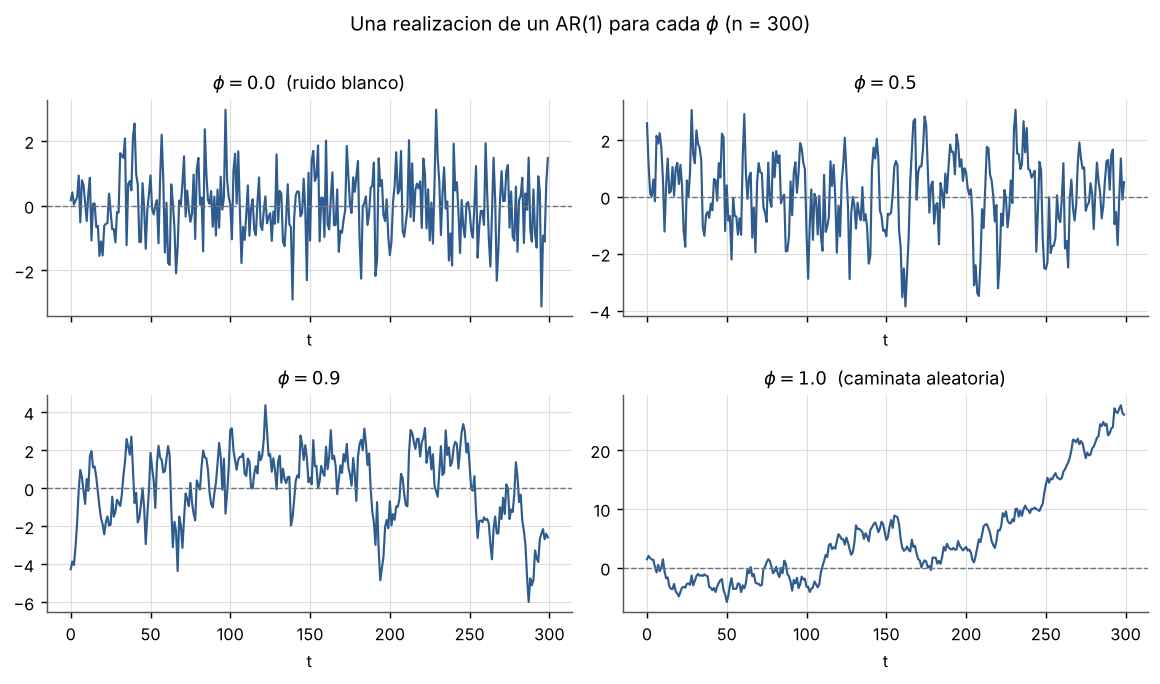
\includegraphics[width=\textwidth]{../figuras/p0_realizaciones.png}
\caption{Una realizaci\'on de un AR(1) para cada~$\phi$. \textbf{Qu\'e
muestra:} con $\phi=0$ la serie es ruido blanco y cruza el cero todo el
tiempo; con $\phi=0.5$ aparecen rachas cortas; con $\phi=0.9$ las rachas son
largas y la serie tarda en volver a su media; con $\phi=1$ ya no hay media a
la cual volver y la serie se va caminando. \textbf{Por qu\'e importa:} es la
misma serie de ecuaciones con un solo par\'ametro distinto, y produce cuatro
comportamientos cualitativamente diferentes.}
\end{figure}

\paragraph{Sobre el descarte con $\phi=1$.} El enunciado advierte que con
$\phi=1$ descartar los primeros \num{200} pasos no logra que el valor
inicial deje de importar, y es cierto: la caminata aleatoria no olvida, as\'i
que al d\'ia \num{200} la serie arranca desde un nivel aleatorio en lugar de
desde cero. \emph{Pero eso no afecta a $r_k$}, porque $r_k$ se calcula sobre
las desviaciones respecto a la media muestral $\bar y$. Sumar una constante
a toda la serie no cambia ni el numerador ni el denominador de
\[
r_k = \frac{\sum_{t=k+1}^{n}(y_t-\bar y)(y_{t-k}-\bar y)}{\sum_{t=1}^{n}(y_t-\bar y)^2}.
\]
El descarte traslada la serie; $r_k$ es invariante a traslaciones.

\begin{table}[htbp]
\centering
\footnotesize
\caption{\textbf{0.2} AR(1) simulado: $n=300$, 5\,000 r\'eplicas por escenario. Cada celda trae el promedio sobre las r\'eplicas y, en peque\~no, su error est\'andar. La banda de la prueba de rezago~1 es $\pm 1.96/\sqrt{300} = 0.1132$.}
\label{tab:p0_tabla_ar1}
\begin{tabular}{ccccccc}
\toprule
\textbf{$\phi$} & \textbf{prom. $r_1$} & \textbf{prom. $r_5$} & \textbf{$\phi^5$ te\'orico} & \textbf{tasa rechazo $|r_1|$} & \textbf{prom. $\hat\phi_{\text{OLS}}$} & \textbf{semilla} \\
\midrule
0.00 & -0.0039 \tiny$\pm$0.0008 & -0.0028 \tiny$\pm$0.0008 & 0.0000 & 0.0500 \tiny$\pm$0.0031 & -0.0039 \tiny$\pm$0.0008 & 2026 \\
0.50 & 0.4892 \tiny$\pm$0.0007 & 0.0199 \tiny$\pm$0.0010 & 0.0312 & 1.0000 \tiny$\pm$0.0000 & 0.4909 \tiny$\pm$0.0007 & 2027 \\
0.90 & 0.8839 \tiny$\pm$0.0004 & 0.5339 \tiny$\pm$0.0014 & 0.5905 & 1.0000 \tiny$\pm$0.0000 & 0.8871 \tiny$\pm$0.0004 & 2028 \\
1.00 & 0.9758 \tiny$\pm$0.0002 & 0.8835 \tiny$\pm$0.0009 & 1.0000 & 1.0000 \tiny$\pm$0.0000 & 0.9824 \tiny$\pm$0.0002 & 2029 \\
\bottomrule
\end{tabular}
\\[0.3em]{\scriptsize \textbf{Qu\'e leer:} con $\phi=0$ la tasa de rechazo es exactamente el 5\,\% nominal. Con $\phi=1$, $r_5=0.88$ en vez del $\phi^5=1$ te\'orico, porque la f\'ormula supone estacionariedad. Y $\hat\phi_{\text{OLS}}$ est\'a sesgado hacia abajo, cada vez m\'as conforme $\phi\to1$.}
\end{table}


\paragraph{0.3 Con $\phi = 0$, {\normalfont\itshape \,¿la tasa de rechazo es
la que esperaban?}} S\'i, y es tranquilizador. Se obtuvo
\num{0.0500} contra el \num{0.05} te\'orico (error est\'andar
\num{0.0031}). Esto es exactamente lo que \emph{debe} pasar: bajo ruido
blanco, $r_1 \approx \mathcal{N}(0, 1/n)$, as\'i que la probabilidad de que
$|r_1|$ se salga de la banda $\pm 1.96/\sqrt{n}$ es del \SI{5}{\percent} por
construcci\'on. Una prueba al \SI{5}{\percent} rechaza el
\SI{5}{\percent} de las veces cuando la hip\'otesis nula es verdadera; eso no
es un defecto, es la definici\'on del nivel de significancia. Esta cifra es
la calibraci\'on de la prueba y sirve de referencia para leer todo lo
dem\'as.

\paragraph{0.3 Para la caminata aleatoria, {\normalfont\itshape ¿qu\'e pasa
con $r_5$ comparado con la teor\'ia $\phi^5 = 1$?}} La teor\'ia dice
$\rho_5 = 1$, pero el promedio muestral es \num{0.8835}, muy por debajo. La
raz\'on es que la f\'ormula $\rho_k = \phi^k$ se deriv\'o \emph{suponiendo
estacionariedad}, y la caminata aleatoria no lo es: ni siquiera tiene una
media poblacional a la cual restar. Al calcular $r_5$ se resta la media
\emph{muestral} del tramo observado, que es un n\'umero distinto en cada
r\'eplica y que absorbe parte del movimiento de la serie. El resultado es un
$r_k$ sistem\'aticamente menor que~1 y que adem\'as decae conforme crece~$k$,
cuando la teor\'ia dir\'ia que se queda clavado en~1.

\paragraph{0.3 {\normalfont\itshape ¿Es consistente el estimado OLS de
$\phi$ con el verdadero, o ven un sesgo?}} Hay sesgo, y es hacia abajo. El
patr\'on es claro en la tabla: con $\phi=0$ el estimado promedio es
\num{-0.0039} (pr\'acticamente insesgado), con $\phi=0.5$ es \num{0.4909},
con $\phi=0.9$ es \num{0.8871} y con $\phi=1$ es \num{0.9824}. El sesgo
crece conforme $\phi$ se acerca a~1: de $\num{0.004}$ a $\num{0.009}$,
$\num{0.013}$ y $\num{0.018}$. Los errores est\'andar de esos promedios son
del orden de \num{0.0008}, as\'i que el sesgo es decenas de veces mayor que
el ruido de simulaci\'on: no es casualidad.

La raz\'on es que en una regresi\'on de $y_t$ contra $y_{t-1}$ el regresor
\emph{no} es fijo: est\'a correlacionado con los errores pasados. Eso rompe
el supuesto que hace insesgado al OLS. El efecto es peque\~no cuando la
memoria es corta, pero se agrava cerca de la ra\'iz unitaria; es el mismo
fen\'omeno que hace que las pruebas de ra\'iz unitaria tipo Dickey--Fuller
necesiten tablas propias en vez de la distribuci\'on normal. En la
pr\'actica significa que, al estimar un AR en datos muy persistentes, uno
tiende a concluir que la serie es \emph{menos} persistente de lo que
realmente es.

\subsection{0.4 Las dos razones para reprobar}

Ahora se simulan procesos \textbf{sin memoria}, $Y_t = m_t + \varepsilon_t$
con $\varepsilon_t$ iid $\mathcal{N}(0,1)$, pero cuya media cambia con el
tiempo.

\begin{figure}[htbp]
\centering
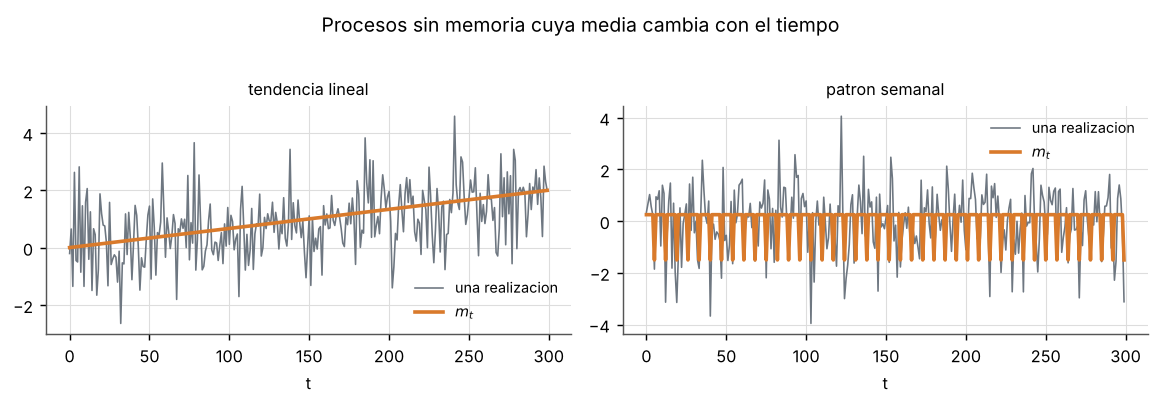
\includegraphics[width=\textwidth]{../figuras/p0_medias_moviles.png}
\caption{Los dos procesos de 0.4. \textbf{Qu\'e muestra:} en gris una
realizaci\'on, en naranja la media $m_t$ que la genera. Entre un punto y el
siguiente no hay ninguna dependencia: cada $\varepsilon_t$ es independiente
de todos los dem\'as. \textbf{Por qu\'e importa:} estas dos series no tienen
memoria y, aun as\'i, reprueban la prueba de ruido blanco.}
\end{figure}

\begin{table}[htbp]
\centering
\footnotesize
\caption{\textbf{0.4} Procesos \emph{sin memoria} cuya media cambia con el tiempo. 5\,000 r\'eplicas de $n=300$ por escenario.}
\label{tab:p0_tabla_media_no_constante}
\begin{tabular}{lcccc}
\toprule
\textbf{escenario} & \textbf{prom. $r_1$} & \textbf{prom. $r_7$} & \textbf{tasa rechazo $|r_1|$} & \textbf{semilla} \\
\midrule
ruido blanco (phi=0) & -0.0039 \tiny$\pm$0.0008 & -0.0017 \tiny$\pm$0.0008 & 0.0500 \tiny$\pm$0.0031 & 2026 \\
tendencia lineal =2t/300 & 0.2445 \tiny$\pm$0.0008 & 0.2296 \tiny$\pm$0.0008 & 0.9846 \tiny$\pm$0.0017 & 2030 \\
patron semanal =-1.5 si t mod 7 = 6 & -0.0484 \tiny$\pm$0.0008 & 0.2646 \tiny$\pm$0.0008 & 0.1146 \tiny$\pm$0.0045 & 2031 \\
\bottomrule
\end{tabular}
\\[0.3em]{\scriptsize \textbf{Qu\'e leer:} la tendencia reprueba la prueba de rezago~1 el 98.5\,\% de las veces sin tener ninguna memoria. El patr\'on semanal la \emph{pasa} (11.5\,\%) aunque su $r_7=0.26$ delata una estructura enorme: la prueba mira donde no hay nada.}
\end{table}


\paragraph{{\normalfont\itshape ¿Cu\'al reprueba la prueba de retardo~1
aunque no tenga memoria?}} La de \textbf{tendencia lineal}. Rechaza en el
\SI{98.46}{\percent} de las r\'eplicas, con un $r_1$ promedio de
\num{0.2445}. El mecanismo es el que anticipa el enunciado: $\bar y$ no es
la media de nadie. Los d\'ias de la parte alta de la tendencia quedan todos
arriba de~$\bar y$ y sus vecinos tambi\'en, as\'i que el producto
$(y_t-\bar y)(y_{t-1}-\bar y)$ es positivo una y otra vez, y $r_1$ sale
grande. La prueba supone estacionariedad y reprueba porque \emph{ese}
supuesto es falso, no porque exista dependencia.

\paragraph{{\normalfont\itshape ¿Cu\'al la pasa aunque tenga estructura?}}
La del \textbf{patr\'on semanal}. Rechaza en apenas el
\SI{11.46}{\percent} de las r\'eplicas, con $r_1 = \num{-0.0484}$: la prueba
de rezago~1 casi no la ve. Y sin embargo la estructura est\'a ah\'i, enorme:
$r_7 = \num{0.2646}$. La media baja a $-1.5$ cada siete pasos y sube a
$0.25$ el resto, de modo que d\'ias separados por exactamente siete pasos se
parecen mucho, pero d\'ias consecutivos no. La prueba de rezago~1 mira
justo donde no hay nada.

\paragraph{{\normalfont\itshape Con\'ectenlo con RANDU en la Tarea~2:
¿qu\'e tienen en com\'un?}} Que una prueba solo ve lo que mira, y que pasar
una prueba no es evidencia de que no haya estructura. RANDU produce
n\'umeros que lucen uniformes e independientes en una y en dos dimensiones,
y solo al mirarlos en \emph{tres} dimensiones se descubre que caen en quince
planos. El patr\'on semanal es el mismo cuento con otro disfraz: es limpio
en el rezago~1 y culpable en el rezago~7. En ambos casos el generador (o el
proceso) \emph{pasa} la prueba equivocada. La lecci\'on pr\'actica es que
una sola prueba de diagn\'ostico, por bien construida que est\'e, solo cubre
la direcci\'on en la que apunta.

\subsection{0.5 La prueba que s\'i ve}

\begin{table}[htbp]
\centering
\footnotesize
\caption{\textbf{0.5} Tasa de rechazo al 5\,\% de Ljung--Box con $m=10$, frente a la prueba de un solo rezago.}
\label{tab:p0_tabla_ljungbox}
\begin{tabular}{lcc}
\toprule
\textbf{escenario} & \textbf{Ljung--Box $m=10$} & \textbf{prueba de rezago 1} \\
\midrule
ruido blanco (phi=0) & 0.0612 \tiny$\pm$0.0034 & 0.0500 \tiny$\pm$0.0031 \\
tendencia lineal & 1.0000 \tiny$\pm$0.0000 & 0.9846 \tiny$\pm$0.0017 \\
patron semanal & 0.9554 \tiny$\pm$0.0029 & 0.1146 \tiny$\pm$0.0045 \\
\bottomrule
\end{tabular}
\\[0.3em]{\scriptsize \textbf{Qu\'e leer:} el caso semanal es el que cambia. Ljung--Box lo rechaza el 95.5\,\% de las veces contra el 11.5\,\% de la prueba de rezago~1, porque $Q(10)$ incluye el rezago~7 en la suma.}
\end{table}


\paragraph{{\normalfont\itshape ¿Qu\'e cambia respecto a la prueba de
retardo~1? ¿Por qu\'e?}} Cambia el caso semanal, y de forma dram\'atica: la
prueba de rezago~1 lo deja pasar el \SI{88.5}{\percent} de las veces,
mientras que Ljung--Box con $m=10$ lo rechaza el \SI{95.54}{\percent} de las
veces. La raz\'on es puramente de cobertura: $Q(10)$ suma
$r_1^2,\dots,r_{10}^2$ en un solo estad\'istico, as\'i que el rezago~7 entra
a la suma y el $r_7 = \num{0.2646}$ se hace notar. La prueba de rezago~1 ni
siquiera lo calcula.

Para el ruido blanco, Ljung--Box rechaza en el \SI{6.12}{\percent} de las
r\'eplicas, razonablemente cerca del \SI{5}{\percent} nominal (con $n=300$ y
$m=10$ la aproximaci\'on $\chi^2$ es buena, aunque no exacta). Y para la
tendencia rechaza siempre, igual que la prueba de rezago~1.

Lo que esto ense\~na, y que se aplicar\'a directamente en las Partes~3 y~4,
es que conviene juntar rezagos en vez de mirarlos de uno en uno. Con
\num{20} rezagos mirados individualmente al \SI{5}{\percent} se espera que
uno se salga por pura suerte; ese es justamente el problema de
comparaciones m\'ultiples que las pruebas portmanteau resuelven. Sobre
cu\'antos rezagos usar, los dos libros discrepan: FPP2 recomienda $m=10$ sin
estacionalidad y $m=2s$ con ella (sin pasar de $n/5$), mientras que Tsay cita
simulaciones que favorecen $m \approx \log(n)$. En esta tarea se reportan
ambos extremos, $Q(6)$ y $Q(12)$, y en los datos reales llevan a la misma
conclusi\'on en todos los casos salvo uno, que se se\~nala en su momento.

% ===========================================================================
\section{Parte 1: Limpieza}
% ===========================================================================

\subsection{1.1 Qu\'e hay en el archivo}

\begin{table}[htbp]
\centering
\footnotesize
\caption{\textbf{1.1} El archivo antes de limpiar.}
\label{tab:p1_conteos}
\begin{tabular}{lr}
\toprule
\textbf{concepto} & \textbf{valor} \\
\midrule
filas & 541909 \\
facturas distintas & 25900 \\
productos distintos (StockCode) & 4070 \\
clientes distintos (CustomerID) & 4372 \\
paises & 38 \\
filas sin CustomerID & 135080 \\
fraccion de filas sin CustomerID & 0.2493 \\
primera fecha & 2010-12-01 08:26:00 \\
ultima fecha & 2011-12-09 12:50:00 \\
venta bruta sin limpiar (GBP) & 9747747.93 \\
\bottomrule
\end{tabular}
\\[0.3em]{\scriptsize \textbf{Qu\'e leer:} una cuarta parte de las filas no tiene cliente identificado; qu\'e hacer con ellas es la decisi\'on m\'as delicada de la limpieza.}
\end{table}


Una cuarta parte de las filas, el \SI{24.93}{\percent}, no tiene
\texttt{CustomerID}. Esa fracci\'on es demasiado grande para ignorarla y la
decisi\'on sobre qu\'e hacer con ella se discute en el inciso~1.2(f).

\paragraph{Por qu\'e leer \texttt{InvoiceNo}, \texttt{StockCode} y
\texttt{CustomerID} como texto.} El enunciado da el consejo y pide
averiguar por qu\'e. Son tres razones distintas:
\begin{itemize}[nosep,leftmargin=1.4em]
  \item \texttt{InvoiceNo} trae prefijos de letra (\texttt{C} de
  cancelaci\'on, \texttt{A} de ajuste). No es un n\'umero, es una etiqueta.
  Le\'ido como n\'umero, pandas se rinde y lo deja como texto mezclado, o
  peor, descarta los prefijos.
  \item \texttt{StockCode} mezcla d\'igitos con letras: \texttt{22423} pero
  tambi\'en \texttt{22423H}, \texttt{POST}, \texttt{DCGS0003}. El sufijo de
  letra distingue variantes de un mismo producto y perderlo fusionar\'ia
  productos distintos.
  \item \texttt{CustomerID} es un identificador, no una cantidad: no tiene
  sentido promediarlo. Y como tiene faltantes, pandas lo convierte a
  \texttt{float}, con lo que el cliente \num{17850} aparece como
  \texttt{17850.0}. Al cruzarlo despu\'es contra una tabla donde est\'a como
  texto, no empata nada y el error es silencioso.
\end{itemize}

\subsection{1.2 Los seis casos, uno por uno}

\begin{table}[htbp]
\centering
\footnotesize
\caption{\textbf{1.2} Los seis casos del enunciado, con su tama\~no y la decisi\'on tomada. La justificaci\'on de cada uno est\'a en el texto.}
\label{tab:p1_casos}
\begin{tabular}{p{8.3cm}rrl}
\toprule
\textbf{caso} & \textbf{filas} & \textbf{monto (\pounds)} & \textbf{decisi\'on} \\
\midrule
(a) filas duplicadas exactas & 5\,268 & 21\,741 & \textbf{SE VAN} \\
(b) facturas con prefijo 'A' & 3 & -11\,062 & \textbf{SE VAN} \\
(b) facturas con prefijo 'C' & 9\,288 & -896\,812 & \textbf{SE QUEDAN} \\
(c) StockCode que no es venta (AMAZONFEE, BANK CHARGES, CRUK, B, S) & 153 & -250\,741 & \textbf{SE VAN} \\
(c) StockCode especial que SI es venta (POST, DOT, C2, D, M, PADS, gift\ & 2\,763 & 205\,094 & \textbf{SE QUEDAN} \\
(d) precio unitario igual a cero & 2\,515 & 0 & \textbf{SE VAN} \\
(d) precio unitario negativo & 2 & -22\,124 & \textbf{SE VAN} \\
(e) cantidad negativa en factura que no es cancelacion & 1\,336 & 0 & \textbf{SE VAN} \\
(f) filas sin CustomerID & 135\,080 & 1\,447\,682 & \textbf{SE QUEDAN (para la serie)} \\
\bottomrule
\end{tabular}
\\[0.3em]{\scriptsize \textbf{Qu\'e leer:} las dos decisiones de \emph{conservar} son tan importantes como las de eliminar. Las cancelaciones deben restar el d\'ia en que ocurren, y las filas sin cliente son 1.45 millones de libras de venta real.}
\end{table}


La decisi\'on de fondo es siempre la misma pregunta: \emph{¿esta l\'inea es
dinero que un cliente pag\'o (o dej\'o de pagar) por algo que la tienda le
vendi\'o?} Si la respuesta es s\'i, la l\'inea se queda aunque el monto sea
negativo. Si es un ajuste contable, un cargo de un tercero o un movimiento de
inventario, se va.

\paragraph{(a) Duplicados exactos.} \num{5268} filas id\'enticas car\'acter
por car\'acter: misma factura, mismo producto, misma cantidad, mismo minuto.
Dos clientes no compran lo mismo en el mismo segundo de la misma factura; es
un error de captura o de exportaci\'on. \textbf{Se van}, conservando la
primera aparici\'on. Si se dejaran, su monto se contar\'ia dos veces.

\paragraph{(b) Facturas que no empiezan con d\'igito.} Hay dos prefijos.
Las \num{9288} filas con \texttt{C} son cancelaciones y \textbf{se quedan},
porque el enunciado pide expresamente que resten el d\'ia en que ocurren.
Las tres filas con \texttt{A} dicen \texttt{Adjust bad debt} y son ajustes
contables por deuda incobrable, con montos de $\pm$\gbp\num{11062}: no son
una venta ni la cancelaci\'on de una venta, sino un movimiento del libro
mayor. \textbf{Se van}.

\paragraph{(c) \texttt{StockCode} que no son productos.} Aqu\'i el
enunciado advierte que no todos son iguales, y en efecto hay tres grupos.
\begin{itemize}[nosep,leftmargin=1.4em]
  \item \textbf{S\'i son productos, aunque el c\'odigo sea raro}:
  \texttt{DCGS*} (bolsas de fiesta, collares de perro, una l\'ampara),
  \texttt{PADS}, y los vales de regalo \texttt{gift\_0001\_*}. \textbf{Se
  quedan}.
  \item \textbf{No son productos pero s\'i son venta}: \texttt{POST},
  \texttt{DOT} y \texttt{C2} son cargos de env\'io que el cliente paga, y
  suman \gbp\num{279462} de ingreso; \texttt{D} es un descuento, que reduce
  leg\'itimamente la venta neta. \textbf{Se quedan}.
  \item \textbf{No son venta}: \texttt{AMAZONFEE} y \texttt{CRUK} son
  comisiones que cobran terceros, \texttt{BANK CHARGES} son cargos del banco,
  \texttt{B} es otro ajuste de deuda incobrable y \texttt{S} son muestras que
  salen de inventario sin venderse. Son gastos o movimientos de bodega, no
  dinero que entr\'o por una venta. \textbf{Se van} (\num{149} filas).
\end{itemize}

\textbf{El caso de \texttt{M} (Manual) merece p\'arrafo propio}, porque es
donde est\'a la trampa. Es tentador borrarlo por ambiguo: son
\num{571} l\'ineas capturadas a mano cuya descripci\'on es simplemente
\texttt{Manual}. Pero borrarlo ser\'ia un error, y el inciso~1.4 lo
demuestra: la factura \texttt{C556445} es una l\'inea \texttt{Manual} de
$-$\gbp\num{38970} que cancela la cesta de picnic de la factura
\texttt{556444} del mismo d\'ia. Si se elimina \texttt{M}, la venta de
\gbp\num{38970} se queda hu\'erfana y aparece un pico falso en la serie.
\textbf{Se queda}.

\paragraph{(d) Precios cero o negativos.} Hay \num{2515} filas con precio
exactamente cero. No aportan nada a la venta neta y \num{1454} de ellas ni
siquiera tienen descripci\'on; el resto dice \texttt{check}, \texttt{damages},
\texttt{?}. Son movimientos de bodega. \textbf{Se van}. Los dos precios
negativos son las facturas \texttt{A} de deuda incobrable, que la regla~(b)
ya se hab\'ia llevado.

\paragraph{(e) Cantidades negativas en facturas que no son cancelaci\'on.}
Son \num{1336} filas, y la columna \texttt{Description} las delata:
\texttt{damages}, \texttt{check}, \texttt{?}, \texttt{thrown away},
\texttt{Unsaleable, destroyed.}, \texttt{wet pallet}, \texttt{smashed}. No
son devoluciones de clientes sino ajustes de inventario que alguien anot\'o a
mano. Un detalle importante: \textbf{las \num{1336} tienen precio cero}, as\'i
que su monto es exactamente \gbp\num{0.00} y quitarlas no mueve ni una libra
de la serie. S\'i mueve los conteos, y por eso importa el orden de las
reglas. \textbf{Se van}.

\paragraph{(f) Filas sin \texttt{CustomerID}.} Esta es la \'unica regla
cuya respuesta depende de para qu\'e se vaya a usar el dato, y el enunciado
lo advierte.

Para la \textbf{serie de ventas}: una transacci\'on sin cliente identificado
sigue siendo dinero que entr\'o a la caja. Son el \SI{24.93}{\percent} de las
filas y alrededor de \gbp\num{1.45} millones. Borrarlas mutilar\'ia la serie
que se quiere pronosticar y, peor, la mutilar\'ia de forma no aleatoria: el
canal de venta sin cliente registrado probablemente no se comporta igual que
el canal mayorista. \textbf{Se quedan}.

Para la \textbf{Parte~6}: ah\'i la pregunta es \emph{qui\'en} compr\'o, y una
venta sin cliente no se le puede asignar a nadie. Un cliente an\'onimo no
tiene recencia ni frecuencia. \textbf{Ah\'i s\'i se excluyen}, y por eso la
funci\'on \texttt{limpiar} solo las \emph{marca} en vez de eliminarlas: la
decisi\'on se toma donde se conoce el uso.

\subsection{1.3 La bit\'acora de limpieza}

\begin{table}[htbp]
\centering
\footnotesize
\caption{\textbf{1.3} Bit\'acora de limpieza. El orden en que se aplican las reglas es parte de la bit\'acora.}
\label{tab:p1_bitacora}
\begin{tabular}{clrr}
\toprule
\textbf{orden} & \textbf{regla} & \textbf{filas eliminadas} & \textbf{monto (\pounds)} \\
\midrule
1 & R1 duplicados exactos & 5\,268 & 21\,740.98 \\
2 & R2 facturas con prefijo distinto de digito o C & 3 & -11\,062.06 \\
3 & R3 StockCode que no es venta al cliente & 149 & -239\,669.22 \\
4 & R4 precio unitario <= 0 & 2\,510 & 0.00 \\
5 & R5 cantidad negativa sin factura de cancelacion & 0 & 0.00 \\
6 & R6 filas sin CustomerID (SE QUEDAN) & 0 & 0.00 \\
7 & TOTAL & 7\,930 & -228\,990.30 \\
\bottomrule
\end{tabular}
\\[0.3em]{\scriptsize \textbf{Qu\'e leer:} R5 elimina cero filas porque R4 ya se llev\'o las 1\,336 filas de cantidad negativa, que ten\'ian todas precio cero. La tabla siguiente muestra qu\'e pasa si se invierte el orden.}
\end{table}


\paragraph{El orden cambia los conteos.} El enunciado lo advierte y conviene
demostrarlo, no solo mencionarlo. Si la regla de cantidades negativas se
aplica \emph{antes} que la de precio cero, en lugar de despu\'es:

\begin{table}[htbp]
\centering
\footnotesize
\caption{\textbf{1.3} Las mismas reglas con R4 y R5 intercambiadas.}
\label{tab:p1_bitacora_orden_alterno}
\begin{tabular}{clrr}
\toprule
\textbf{orden} & \textbf{regla} & \textbf{filas eliminadas} & \textbf{monto (\pounds)} \\
\midrule
1 & R1 duplicados exactos & 5\,268 & 21\,740.98 \\
2 & R2 prefijo distinto de digito o C & 3 & -11\,062.06 \\
3 & R3 StockCode que no es venta & 149 & -239\,669.22 \\
4 & R5 cantidad negativa sin cancelacion (ADELANTADA) & 1\,336 & 0.00 \\
5 & R4 precio <= 0 (ATRASADA) & 1\,174 & 0.00 \\
\bottomrule
\end{tabular}
\\[0.3em]{\scriptsize \textbf{Qu\'e leer:} la misma regla elimina 1\,336 filas aqu\'i y 0 en la tabla anterior. El conjunto final es id\'entico (533\,979 filas), pero la bit\'acora cuenta otra historia: sin el orden documentado no es reproducible.}
\end{table}


La misma regla elimina \num{1336} filas en un orden y \num{0} en el otro,
porque las \num{1336} filas de cantidad negativa tienen todas precio cero y
quien llegue primero se las lleva. El conjunto final es id\'entico en ambos
\'ordenes (\num{533979} filas), pero la bit\'acora cuenta dos historias
distintas. Es un buen recordatorio de que una bit\'acora de limpieza sin el
orden documentado no es reproducible.

\subsection{1.4 Las seis l\'ineas m\'as grandes}

\begin{table}[htbp]
\centering
\footnotesize
\caption{\textbf{1.4} Las seis l\'ineas de mayor $|$Quantity $\times$ UnitPrice$|$ \emph{antes} de limpiar.}
\label{tab:p1_extremos}
\begin{tabular}{llrrlc}
\toprule
\textbf{factura} & \textbf{descripci\'on} & \textbf{cantidad} & \textbf{monto (\pounds)} & \textbf{fecha y hora} & \textbf{sobrevive} \\
\midrule
C581484 & PAPER CRAFT , LITTLE BIRDI & -80\,995 & -168\,469.60 & 2011-12-09 09:27 & s\'i \\
581483 & PAPER CRAFT , LITTLE BIRDI & 80\,995 & 168\,469.60 & 2011-12-09 09:15 & s\'i \\
541431 & MEDIUM CERAMIC TOP STORAGE & 74\,215 & 77\,183.60 & 2011-01-18 10:01 & s\'i \\
C541433 & MEDIUM CERAMIC TOP STORAGE & -74\,215 & -77\,183.60 & 2011-01-18 10:17 & s\'i \\
556444 & PICNIC BASKET WICKER 60 PI & 60 & 38\,970.00 & 2011-06-10 15:28 & s\'i \\
C556445 & Manual & -1 & -38\,970.00 & 2011-06-10 15:31 & s\'i \\
\bottomrule
\end{tabular}
\\[0.3em]{\scriptsize \textbf{Qu\'e leer:} son tres pares venta/cancelaci\'on, no seis eventos. Las seis sobreviven a la limpieza porque ninguna es un error; lo que las resuelve es netear por d\'ia, ya que en los tres casos la cancelaci\'on ocurre el mismo d\'ia (12, 16 y 3 minutos despu\'es).}
\end{table}


Son tres pares, no seis eventos independientes, y los tres cuentan la misma
historia:

\begin{enumerate}[leftmargin=1.5em]
  \item \textbf{\texttt{581483} / \texttt{C581484}}, \num{80995} unidades de
  \texttt{PAPER CRAFT, LITTLE BIRDIE} por \gbp\num{168470}. La venta se
  registra el 9 de diciembre a las 09:15 y se cancela a las 09:27, doce
  minutos despu\'es, el mismo d\'ia. Es el pedido m\'as grande de todo el
  archivo y nunca existi\'o de verdad.
  \item \textbf{\texttt{541431} / \texttt{C541433}}, \num{74215} tarros de
  cer\'amica por \gbp\num{77184}. Vendidos el 18 de enero a las 10:01,
  cancelados a las 10:17.
  \item \textbf{\texttt{556444} / \texttt{C556445}}, una cesta de picnic por
  \gbp\num{38970}. Vendida el 10 de junio a las 15:28 y cancelada a las
  15:31, pero \emph{la cancelaci\'on viene como una l\'inea
  \texttt{Manual}}, no como el mismo producto.
\end{enumerate}

\paragraph{{\normalfont\itshape ¿Su limpieza las resuelve?}} \textbf{No, y
no deber\'ia.} Las seis l\'ineas sobreviven a las seis reglas, porque las
seis son ventas o cancelaciones leg\'itimas: tienen precio positivo,
c\'odigo de producto v\'alido y factura con formato correcto. No hay nada en
la l\'inea, vista de forma aislada, que permita se\~nalarla como error. Una
regla del tipo ``elimine cantidades mayores a \num{10000}'' ser\'ia
arbitraria y borrar\'ia tambi\'en pedidos mayoristas genuinos.

\paragraph{{\normalfont\itshape ¿Las resuelve el hecho de netear por
d\'ia?}} \textbf{S\'i, en los tres casos, y de forma exacta.} En los tres
pares la venta y su cancelaci\'on caen en el \emph{mismo d\'ia} calendario
(separadas por 12 minutos, 16 minutos y 3 minutos respectivamente), as\'i que
al sumar todas las l\'ineas del d\'ia los montos se anulan y la serie diaria
ni se entera. Esto es exactamente lo que justifica la definici\'on de venta
neta diaria del enunciado.

Vale la pena notar d\'onde \emph{no} funcionar\'ia: si una cancelaci\'on
ocurriera varios d\'ias despu\'es de la venta, el neteo diario dejar\'ia un
pico positivo un d\'ia y un hoyo negativo otro, y ninguno de los dos
ser\'ia real. Con estos datos los pares grandes son todos del mismo d\'ia,
pero no hay garant\'ia de que lo sean en general.

\subsection{1.5 La funci\'on \texttt{limpiar}}

Toda la limpieza est\'a escrita como una sola funci\'on
\texttt{limpiar(df)} en \texttt{src/limpieza.py}, su propio archivo, tal
como pide el enunciado. Devuelve el \texttt{DataFrame} limpio con dos
columnas nuevas (\texttt{monto} y \texttt{cancelacion}) y, opcionalmente, la
bit\'acora. Se reusa tal cual en la Parte~6 y queda disponible para el
Proyecto~1.

% ===========================================================================
\section{Parte 2: El calendario}
% ===========================================================================

\begin{table}[htbp]
\centering
\footnotesize
\caption{\textbf{2.1--2.4} El calendario de la serie.}
\label{tab:p2_resumen_calendario}
\begin{tabular}{lr}
\toprule
\textbf{concepto} & \textbf{valor} \\
\midrule
primer dia & 2010-12-01 \\
ultimo dia de los datos & 2011-12-09 \\
dias calendario (inclusive) & 374 \\
dias con al menos una transaccion & 305 \\
dias sin transacciones & 69 \\
   de ellos, sabados & 53 \\
   de ellos, feriados bancarios & 11 \\
   sin explicacion & 5 \\
serie final: dias en el calendario (sin el ultimo dia) & 373 \\
serie final: dias abiertos & 304 \\
venta neta total de la serie (GBP) & 9944626.32 \\
\bottomrule
\end{tabular}
\\[0.3em]{\scriptsize \textbf{Qu\'e leer:} de 374 d\'ias calendario solo 305 tuvieron ventas. Los 53 s\'abados son el hallazgo que fija $s=6$ en la Parte~4.}
\end{table}


\subsection{2.1 Cu\'antos d\'ias hay y cu\'antos se usaron}

Entre el 1 de diciembre de 2010 y el 9 de diciembre de 2011, ambos
inclusive, hay \textbf{\num{374} d\'ias calendario}. De esos,
\textbf{\num{305} tuvieron al menos una transacci\'on} y \num{69} no
tuvieron ninguna.

\subsection{2.2 Los d\'ias sin transacciones}

\paragraph{{\normalfont\itshape ¿Qu\'e d\'ia de la semana no abre la
tienda?}} El \textbf{s\'abado}. De los \num{69} d\'ias sin transacciones,
\num{53} son s\'abados, y no hay ni un solo s\'abado con ventas en todo el
a\~no. Vale la pena subrayar que la tienda \textbf{s\'i abre los domingos}
(\num{50} domingos con ventas), que es lo contrario de lo que uno
supondr\'ia por costumbre. \textbf{Esto tiene una consecuencia directa sobre
el resto de la tarea: la semana comercial tiene seis d\'ias, no siete, y por
eso el per\'iodo estacional de los modelos SARIMA de la Parte~4 es $s=6$ y
no $s=7$.}

\paragraph{{\normalfont\itshape ¿Qu\'e otros d\'ias faltan y qu\'e
fueron?}} Los \num{16} restantes se reparten entre \num{11} feriados
bancarios del Reino Unido y \num{5} d\'ias del cierre navide\~no de fin de
a\~no (del 30 de diciembre de 2010 al 2 de enero de 2011, m\'as el domingo
de Pascua).

\begin{table}[htbp]
\centering
\footnotesize
\caption{\textbf{2.2} Los d\'ias sin transacciones que \emph{no} son s\'abado. Los 53 s\'abados se omiten de la tabla por brevedad.}
\label{tab:p2_feriados}
\begin{tabular}{llll}
\toprule
\textbf{fecha} & \textbf{d\'ia} & \textbf{motivo} & \textbf{tipo} \\
\midrule
2010-12-24 & viernes & feriado bancario: Nochebuena (la tienda cierra & fijo \\
2010-12-26 & domingo & feriado bancario: Boxing Day & fijo \\
2010-12-27 & lunes & feriado bancario: Navidad (dia sustituto) & fijo \\
2010-12-28 & martes & feriado bancario: Boxing Day (dia sustituto) & fijo \\
2010-12-29 & miercoles & sin explicacion en el calendario & --- \\
2010-12-30 & jueves & sin explicacion en el calendario & --- \\
2010-12-31 & viernes & sin explicacion en el calendario & --- \\
2011-01-02 & domingo & sin explicacion en el calendario & --- \\
2011-01-03 & lunes & feriado bancario: Ano Nuevo (dia sustituto) & fijo \\
2011-04-22 & viernes & feriado bancario: Viernes Santo & \textbf{MOVIL} \\
2011-04-24 & domingo & sin explicacion en el calendario & --- \\
2011-04-25 & lunes & feriado bancario: Lunes de Pascua & \textbf{MOVIL} \\
2011-04-29 & viernes & feriado bancario: Boda real (feriado extraordi & \textbf{irrepetible} \\
2011-05-02 & lunes & feriado bancario: Early May Bank Holiday & fijo (primer lunes de mayo) \\
2011-05-30 & lunes & feriado bancario: Spring Bank Holiday & fijo (ultimo lunes de mayo) \\
2011-08-29 & lunes & feriado bancario: Summer Bank Holiday & fijo (ultimo lunes de agosto) \\
\bottomrule
\end{tabular}
\\[0.3em]{\scriptsize \textbf{Qu\'e leer:} tres de los feriados son m\'oviles o irrepetibles. La Pascua se mueve hasta un mes entre a\~nos y la boda real de 2011 no se repite nunca, as\'i que ning\'un modelo entrenado con un a\~no de datos puede anticiparlos.}
\end{table}


\paragraph{{\normalfont\itshape ¿Cu\'ales de los que encontraron son
m\'oviles?}} Tres, y es justo la advertencia de FPP2 \S12.1 sobre los
feriados m\'oviles:
\begin{itemize}[nosep,leftmargin=1.4em]
  \item El \textbf{Viernes Santo} (22 de abril de 2011) y el \textbf{Lunes
  de Pascua} (25 de abril) se mueven con la Pascua, que puede caer entre el
  22 de marzo y el 25 de abril. En 2011 cay\'o muy tarde; en 2012 fue el 6 y
  el 9 de abril. Un modelo que aprenda ``la tercera semana de abril se vende
  poco'' con un a\~no de datos estar\'a equivocado al a\~no siguiente.
  \item La \textbf{boda real} del 29 de abril de 2011 es peor que m\'ovil:
  es \textbf{irrepetible}. Fue un feriado extraordinario decretado para ese
  a\~no. No hay forma de que ning\'un modelo lo anticipe, y tampoco deber\'ia
  intentarlo.
\end{itemize}
Los dem\'as son fijos por regla (primer lunes de mayo, \'ultimo lunes de mayo,
\'ultimo lunes de agosto) o por fecha (Navidad, Boxing Day), as\'i que s\'i
se pueden poner en el calendario por adelantado. Esa es la raz\'on por la
cual, en la Parte~5, se permite saber de antemano qu\'e d\'ias futuros est\'an
abiertos: es informaci\'on de calendario, no informaci\'on del futuro.

\subsection{2.3 {\normalfont\itshape ¿Un d\'ia sin transacciones es un cero
o un dato faltante?}}

Depende de la pregunta que se le haga a la serie, y las dos lecturas son
correctas en contextos distintos.

\paragraph{Debe ser \textbf{cero} cuando se mide dinero.} Si la pregunta es
``\gbp cu\'anto vendimos esta semana'' o ``\gbp cu\'anto vendimos en
noviembre'', el s\'abado aport\'o exactamente cero libras. Un faltante
obligar\'ia a inventar un n\'umero o a reportar la suma de seis d\'ias como
si fuera de siete. Por eso en el inciso~3.1 la media m\'ovil centrada de
siete d\'ias se calcula \emph{rellenando los d\'ias cerrados con cero}: se
busca el nivel de ingreso de la semana calendario, y un s\'abado cerrado
contribuye cero a ese nivel.

\paragraph{Debe ser \textbf{faltante} cuando se mide comportamiento.} Si la
pregunta es ``\gbp cu\'anto vende un d\'ia t\'ipico'' o ``\gbp qu\'e tan
grande es la autocorrelaci\'on de un d\'ia al siguiente'', meter los
s\'abados como ceros es da\~nino. Jalar\'ian la media hacia abajo, inflar\'ian
la varianza y, sobre todo, meter\'ian una estacionalidad artificial de
per\'iodo~7 que no describe el negocio sino el horario. El s\'abado no es un
d\'ia de venta cero: es un d\'ia que no existe para la tienda. Por eso toda
la modelaci\'on de las Partes~3.3 a~5 trabaja sobre \textbf{d\'ias abiertos,
una fila por d\'ia}, y los d\'ias cerrados quedan marcados como faltantes en
el calendario completo.

\subsection{2.4 {\normalfont\itshape ¿Est\'a completo el \'ultimo d\'ia?}}

\textbf{No.} El 9 de diciembre de 2011 la \'ultima factura es de las
\textbf{12:50}, mientras que en el resto de los d\'ias la \'ultima factura
es, en mediana, de las \textbf{17:00} y nunca antes de las \textbf{15:00}.
El archivo se cort\'o a la mitad de la jornada: la venta registrada
(\gbp\num{32112}) es la de media ma\~nana, no la del d\'ia.

\paragraph{{\normalfont\itshape ¿Qu\'e hacen con \'el?}} \textbf{Se
descarta.} Dejarlo ser\'ia meter un dato bajo que no refleja una ca\'ida de
la demanda sino el final del archivo, y el 8 de diciembre es de todas formas
el \'ultimo d\'ia que el enunciado manda evaluar. La alternativa de
escalarlo (multiplicarlo por la proporci\'on t\'ipica de venta que ocurre
despu\'es de mediod\'ia) inventar\'ia un dato, y para un solo d\'ia al final
de la serie no vale la pena el riesgo.

\begin{figure}[htbp]
\centering
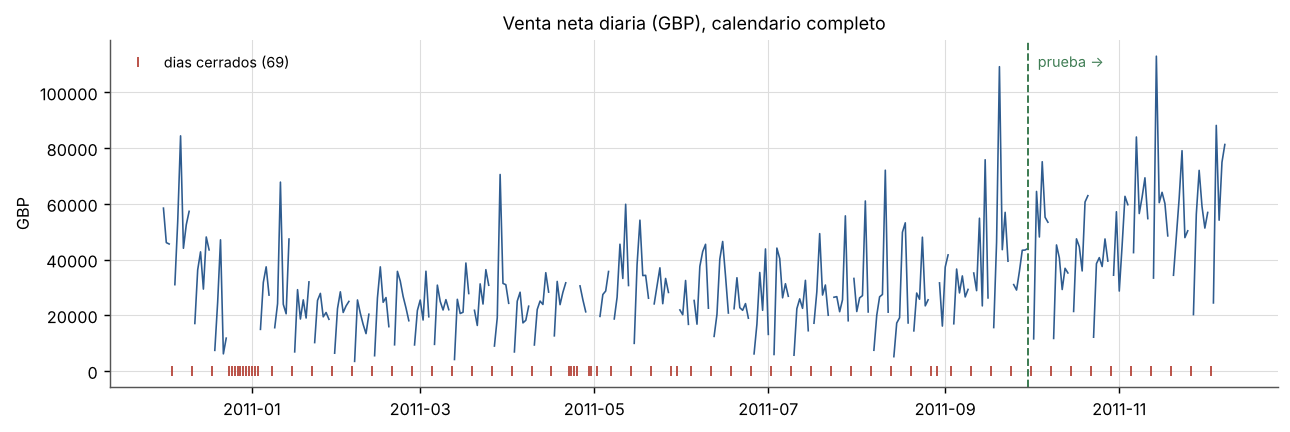
\includegraphics[width=\textwidth]{../figuras/p2_serie.png}
\caption{La serie de venta neta diaria sobre el calendario completo.
\textbf{Qu\'e muestra:} los \num{303} d\'ias del calendario tras descartar
el \'ultimo, con los d\'ias cerrados marcados abajo en rojo y la l\'inea
verde separando entrenamiento de prueba. \textbf{Por qu\'e importa:} se ven
de un vistazo los tres rasgos que gobiernan el resto de la tarea: el hueco
largo de fin de a\~no, el diente de sierra semanal, y la subida clara a
partir de septiembre que hace que el per\'iodo de prueba sea m\'as dif\'icil
que el entrenamiento.}
\end{figure}

De aqu\'i en adelante se trabaja con la serie diaria sobre el calendario
completo, con los d\'ias cerrados marcados como faltantes y sin el \'ultimo
d\'ia. \textbf{Entrenamiento} es todo hasta el 30 de septiembre de 2011
(\num{245} d\'ias abiertos) y \textbf{prueba} son los d\'ias abiertos del 3
de octubre al 8 de diciembre (\num{58} d\'ias evaluados).

% ===========================================================================
\section{Parte 3: Tendencia, estacionalidad y autocorrelaci\'on}
% ===========================================================================

Lo que hacen 3.1 y 3.2 es una \emph{descomposici\'on cl\'asica
multiplicativa}: serie $=$ tendencia $\times$ estacionalidad $\times$ resto.

\subsection{3.1 Tendencia}

\begin{figure}[htbp]
\centering
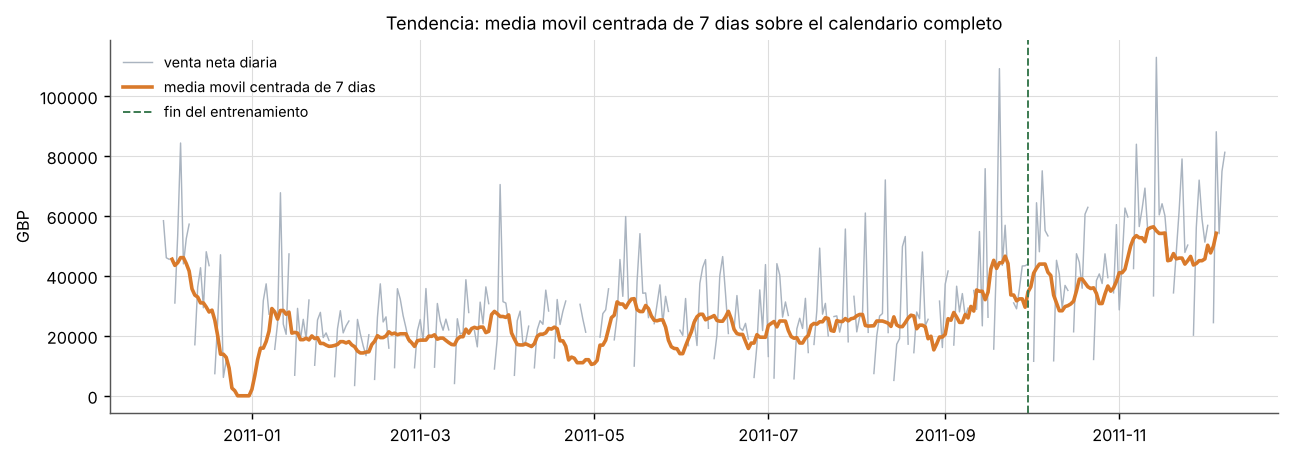
\includegraphics[width=\textwidth]{../figuras/p3_tendencia.png}
\caption{Media m\'ovil centrada de siete d\'ias sobre el calendario
completo, con los d\'ias cerrados rellenados con cero. \textbf{Qu\'e
muestra:} en gris la venta diaria, que sube y baja violentamente; en naranja
la media m\'ovil, que se queda con el nivel. \textbf{Por qu\'e importa:} el
diente de sierra diario desaparece por completo, y lo que queda es una
tendencia plana alrededor de \gbp\num{20000} de enero a julio que empieza a
subir en agosto y se dispara en noviembre. El hoyo de finales de diciembre
no es una ca\'ida de la demanda: es la tienda cerrada nueve d\'ias, y la
media m\'ovil lo registra como ceros.}
\end{figure}

\paragraph{{\normalfont\itshape ¿Por qu\'e 7 y no 5 ni 30?}} Porque siete es
exactamente el largo del ciclo que se quiere eliminar. La semana calendario
dura siete d\'ias, as\'i que una media de siete d\'ias consecutivos contiene
cada d\'ia de la semana exactamente una vez: el jueves bueno y el domingo
malo entran con el mismo peso y el efecto del d\'ia de la semana se cancela
aritm\'eticamente, no por aproximaci\'on. Con cinco d\'ias la ventana
contendr\'ia dos jueves en unas posiciones y ninguno en otras, as\'i que la
media m\'ovil heredar\'ia un residuo del propio patr\'on semanal que
pretende quitar. Con treinta d\'ias s\'i se cancelar\'ia el efecto semanal
(aproximadamente, porque 30 no es m\'ultiplo de 7), pero la ventana ser\'ia
tan ancha que tambi\'en alisar\'ia lo que interesa conservar: la subida de
noviembre quedar\'ia aplastada y desplazada. La regla general es que la
ventana se escoge igual al per\'iodo estacional, ni m\'as ni menos.

\paragraph{{\normalfont\itshape ¿Por qu\'e centrada?}} Para que la
tendencia no quede corrida en el tiempo. Una media m\'ovil hacia atr\'as
asigna al d\'ia~$t$ el promedio de los siete d\'ias que terminan en~$t$, es
decir el nivel del centro de esa ventana, que es $t-3$. Eso retrasa toda la
curva tres d\'ias y har\'ia parecer que la subida de noviembre empez\'o
despu\'es de cuando realmente empez\'o. Centrarla la alinea con la serie.
\textbf{El precio de centrarla es justamente lo que la vuelve ilegal como
predictor}: para calcular la tendencia del d\'ia~$t$ hay que conocer
$y_{t+1}$, $y_{t+2}$ y $y_{t+3}$, que a\'un no han ocurrido. Esta es la
trampa del inciso~5.4 y aqu\'i ya queda sembrada.

\paragraph{La tendencia en dos o tres oraciones.} El nivel se mantiene
notablemente plano alrededor de \gbp\num{20000} diarios desde enero hasta
julio, con oscilaciones pero sin direcci\'on. A partir de agosto empieza una
subida sostenida que lo lleva a unos \gbp\num{30000} al cerrar septiembre,
y que se acelera fuerte en octubre y noviembre hasta un m\'aximo de
\gbp\num{56412} el 13 de noviembre: es la temporada navide\~na de una tienda
de art\'iculos de regalo que vende casi todo a mayoristas, los cuales se
abastecen con semanas de anticipaci\'on. \textbf{La consecuencia pr\'actica
es incomoda y conviene decirla desde ya: el per\'iodo de prueba cae
\'integramente sobre el tramo m\'as alto y m\'as inclinado de la serie,
as\'i que cualquier modelo entrenado solo con datos hasta septiembre va a
quedarse corto.} Eso es exactamente lo que se observa en la Parte~5.

\subsection{3.2 Estacionalidad}

\begin{table}[htbp]
\centering
\footnotesize
\caption{\textbf{3.2} \'Indice estacional por d\'ia de la semana, calculado solo sobre el entrenamiento.}
\label{tab:p3_indices}
\begin{tabular}{lcccc}
\toprule
\textbf{d\'ia} & \textbf{\'indice $y_t/\mathrm{MA}_t$} & \textbf{desv. est.} & \textbf{$n$ d\'ias} & \textbf{normalizado} \\
\midrule
lunes & 1.1688 & 0.3239 & 37 & 0.9736 \\
martes & 1.5471 & 0.5434 & 42 & 1.2887 \\
miercoles & 1.2353 & 0.3866 & 42 & 1.0290 \\
jueves & 1.5579 & 0.4952 & 42 & 1.2977 \\
viernes & 1.1245 & 0.3193 & 39 & 0.9366 \\
domingo & 0.5695 & 0.2997 & 40 & 0.4744 \\
\bottomrule
\end{tabular}
\\[0.3em]{\scriptsize \textbf{Qu\'e leer:} jueves y martes venden m\'as del triple que el domingo. El promedio de los seis \'indices es 1.2005 y no 1 porque el denominador promedia siete d\'ias calendario de los cuales uno es un s\'abado cerrado que entra como cero, lo que lo subestima por un factor de $6/7$.}
\end{table}


\begin{figure}[htbp]
\centering
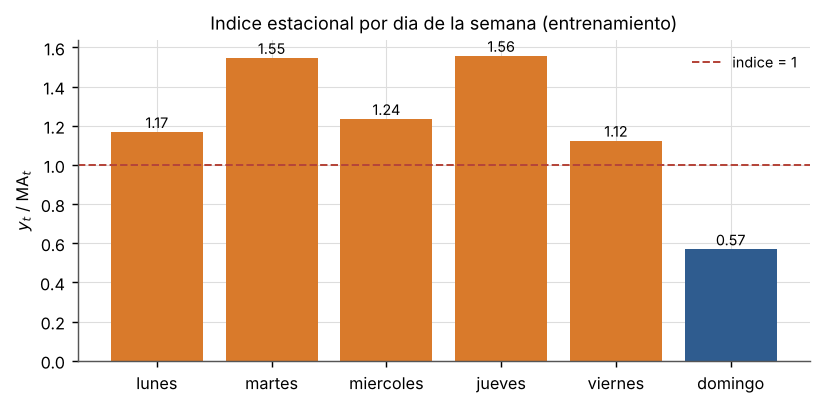
\includegraphics[width=0.72\textwidth]{../figuras/p3_indices.png}
\caption{\'Indice estacional de cada d\'ia de la semana: el promedio, sobre
el entrenamiento, del cociente $y_t/\mathrm{MA}_t$. \textbf{Qu\'e muestra:}
el jueves y el martes venden alrededor de \num{1.55} veces el nivel de la
semana; el domingo apenas \num{0.57}. \textbf{Por qu\'e importa:} la
diferencia entre el mejor y el peor d\'ia es de casi tres a uno, as\'i que
cualquier modelo que ignore el d\'ia de la semana est\'a dejando sobre la
mesa la fuente de variaci\'on m\'as grande y m\'as predecible de la serie.}
\end{figure}

\paragraph{{\normalfont\itshape ¿Qu\'e d\'ias venden m\'as?}}
\textbf{Jueves} (\'indice \num{1.558}) y \textbf{martes} (\num{1.547}), casi
empatados, seguidos de mi\'ercoles (\num{1.235}), lunes (\num{1.169}) y
viernes (\num{1.125}). El \textbf{domingo} es con mucho el m\'as flojo:
\num{0.570}, menos de la mitad del jueves. El patr\'on tiene sentido para un
negocio mayorista: los compradores profesionales hacen sus pedidos entre
semana, con un pico a mitad de semana, y el domingo apenas entra el goteo de
pedidos web de consumidores finales.

\paragraph{{\normalfont\itshape ¿Por qu\'e el promedio de los seis \'indices
no es 1?}} El promedio es \textbf{\num{1.2005}}, no \num{1}, y la raz\'on es
puramente aritm\'etica, no un error. El denominador $\mathrm{MA}_t$ es un
promedio sobre \textbf{siete} d\'ias calendario, pero uno de esos siete es un
s\'abado cerrado que entra como \textbf{cero}. Entonces $\mathrm{MA}_t$
reparte la venta de seis d\'ias entre siete casillas, con lo que subestima
sistem\'aticamente el nivel de un d\'ia abierto por un factor de $6/7$. Al
dividir cada d\'ia abierto entre ese denominador demasiado peque\~no, todos
los cocientes salen inflados por aproximadamente $7/6 = \num{1.1667}$. El
valor observado de \num{1.2005} es cercano a esa cifra; la diferencia que
queda se debe a los feriados (que a\~naden m\'as ceros al denominador en
ciertas semanas) y a que el promedio de cocientes no es el cociente de
promedios. La columna \texttt{indice\_normalizado} de la tabla reescala los
seis \'indices para que promedien~1 y permite leerlos como ``porcentaje
respecto a un d\'ia abierto promedio''.

\subsection{3.3 Autocorrelaci\'on}

La funci\'on $r_k$ est\'a implementada a mano con \texttt{numpy}, es la
misma de la Parte~0, y se aplica sobre los \textbf{\num{245} d\'ias abiertos
del entrenamiento, una fila por d\'ia, sin calendario}.

\begin{figure}[htbp]
\centering
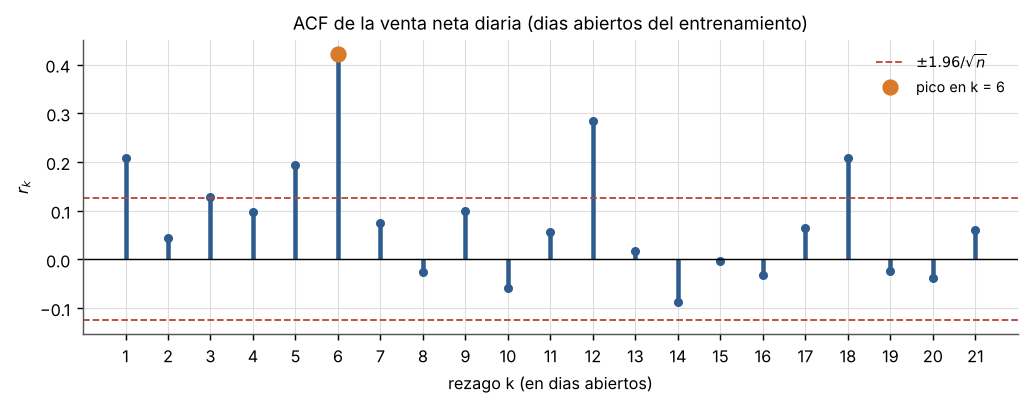
\includegraphics[width=\textwidth]{../figuras/p3_acf.png}
\caption{ACF de la venta neta diaria sobre los d\'ias abiertos del
entrenamiento, con las bandas $\pm 1.96/\sqrt{n}$. \textbf{Qu\'e muestra:}
seis de \num{21} rezagos se salen de las bandas, y el patr\'on no es
aleatorio: los picos est\'an en \num{6}, \num{12} y \num{18}, que son
m\'ultiplos exactos de seis. \textbf{Por qu\'e importa:} esos picos son la
firma de una estacionalidad de per\'iodo~6 en la escala de d\'ias abiertos, y
son la evidencia emp\'irica que justifica usar $s=6$ en los modelos SARIMA de
la Parte~4.}
\end{figure}

\paragraph{{\normalfont\itshape ¿Cu\'antos rezagos se salen?}} \textbf{Seis
de \num{21}}: los rezagos \num{1}, \num{3}, \num{5}, \num{6}, \num{12}
y~\num{18}, contra la banda $\pm\num{0.1252}$. Si la serie fuera ruido
blanco se esperar\'ia que se saliera aproximadamente uno
($21 \times 0.05 \approx 1.05$).

\paragraph{{\normalfont\itshape ¿Pasa la prueba de retardo~1 de la
Tarea~2?}} \textbf{No, la reprueba.} $r_1 = \num{0.2092}$, bastante por
encima de \num{0.1252}. A diferencia del caso semanal simulado de la
Parte~0.4, que s\'i la pasaba, aqu\'i hasta la prueba m\'as miope detecta
que algo pasa.

\paragraph{{\normalfont\itshape ¿En qu\'e rezago est\'a el pico y cu\'antos
d\'ias calendario representa?}} El pico est\'a en \textbf{$k=6$}, con
$r_6 = \num{0.4224}$, el doble que cualquier otro. Y seis d\'ias abiertos
son \textbf{siete d\'ias calendario}: se verific\'o directamente sobre las
fechas y la mediana de la distancia calendario entre un d\'ia abierto y el
sexto anterior es exactamente \num{7} d\'ias (m\'inimo \num{7}, m\'aximo
\num{18} en las semanas con feriados). Es decir, el pico en el rezago~6 es
\textbf{el mismo d\'ia de la semana de la semana anterior}. Los picos
secundarios en \num{12} y~\num{18} son dos y tres semanas atr\'as. Esta es la
traducci\'on exacta del \'indice estacional de 3.2 al lenguaje de la ACF, y
es la raz\'on por la que la parte estacional de los modelos SARIMA usa
$s=6$: en la escala en que se modela, que es d\'ias abiertos, la semana mide
seis.

\paragraph{Ljung--Box.}
\begin{table}[htbp]
\centering
\footnotesize
\caption{\textbf{3.3} Ljung--Box sobre la venta neta de los 245 d\'ias abiertos del entrenamiento.}
\label{tab:p3_ljungbox}
\begin{tabular}{ccccc}
\toprule
\textbf{$m$} & \textbf{$Q(m)$} & \textbf{gl} & \textbf{valor-$p$} & \textbf{rechaza al 5\,\%} \\
\midrule
6 & 72.53 & 6 & 1.24e-13 & \textbf{s\'i} \\
12 & 99.38 & 12 & 7.77e-16 & \textbf{s\'i} \\
\bottomrule
\end{tabular}
\\[0.3em]{\scriptsize \textbf{Qu\'e leer:} los dos criterios de $m$ que discuten FPP2 y Tsay coinciden sin ambig\"uedad: la serie no es ruido blanco.}
\end{table}

Ambas pruebas rechazan de forma aplastante: $Q(6)=\num{72.53}$ con
$p = \num{1.2e-13}$ y $Q(12)=\num{99.38}$ con $p = \num{7.8e-16}$. Los dos
criterios de $m$ que discuten FPP2 y Tsay coinciden sin ambig\"uedad.

\paragraph{3.3(b) {\normalfont\itshape ¿Cu\'anto de esa autocorrelaci\'on es
memoria y cu\'anto es media no constante?}} Con lo visto en la Parte~0, hay
razones para sospechar de ambas y la ACF por s\'i sola no las distingue.

Hay evidencia fuerte de \textbf{media no constante} por dos v\'ias. La
primera es la estacionalidad: 3.2 ya mostr\'o que la media de un jueves es
casi el triple que la de un domingo, as\'i que $\bar y$ no es la media de
nadie, exactamente el mecanismo del caso semanal de 0.4. La segunda es la
tendencia: 3.1 mostr\'o que el nivel sube claramente a partir de agosto, que
es el mecanismo del caso de tendencia lineal de 0.4. Los picos en \num{6},
\num{12} y \num{18} son la firma caracter\'istica de lo primero.

Pero tambi\'en hay se\~nales de \textbf{memoria}: $r_1 = \num{0.2092}$ es
grande y positivo, y el rezago~1 no es m\'ultiplo de seis, as\'i que la
estacionalidad semanal no lo explica de forma obvia. Adem\'as la ACF no cae
r\'apido a cero despu\'es del rezago~6, lo que sugiere algo m\'as que
estacionalidad pura.

La forma honesta de separarlos es la receta cl\'asica, que es justo lo que
hace la Parte~4: primero se quita la media no constante (el d\'ia de la
semana y la tendencia) y despu\'es se mira qu\'e autocorrelaci\'on le queda
al residuo. Lo que sobreviva a ese filtro s\'i es memoria.

% ===========================================================================
\section{Parte 4: Del AR(1) al SARIMA}
% ===========================================================================

Toda esta parte trabaja sobre los \num{245} d\'ias abiertos del
entrenamiento como una fila por d\'ia.

\subsection{4.1 Quitar el d\'ia de la semana}

\begin{table}[htbp]
\centering
\footnotesize
\caption{\textbf{4.1} OLS de la venta contra indicadoras de d\'ia de la semana, sin intercepto. $R^2 = 0.2606$.}
\label{tab:p4_ols_dow}
\begin{tabular}{lrc}
\toprule
\textbf{d\'ia} & \textbf{coeficiente (\pounds)} & \textbf{$n$ d\'ias} \\
\midrule
lunes & 27\,770.41 & 37 \\
martes & 35\,966.22 & 42 \\
miercoles & 28\,504.25 & 43 \\
jueves & 36\,093.53 & 43 \\
viernes & 27\,106.35 & 40 \\
domingo & 13\,819.45 & 40 \\
\bottomrule
\end{tabular}
\\[0.3em]{\scriptsize \textbf{Qu\'e leer:} los coeficientes son la venta promedio de cada d\'ia y reproducen el orden de los \'indices de 3.2. El modelo le asigna el mismo valor a todos los jueves del a\~no, lo que deja la tendencia entera dentro de los residuos.}
\end{table}


Los coeficientes son la venta promedio de cada d\'ia de la semana en libras
y reproducen el orden del inciso~3.2: jueves (\gbp\num{36094}) y martes
(\gbp\num{35966}) arriba, domingo (\gbp\num{13819}) muy abajo. El
$R^2$ es \num{0.2606}: el d\'ia de la semana por s\'i solo explica algo
m\'as de una cuarta parte de la variaci\'on diaria.

\begin{figure}[htbp]
\centering
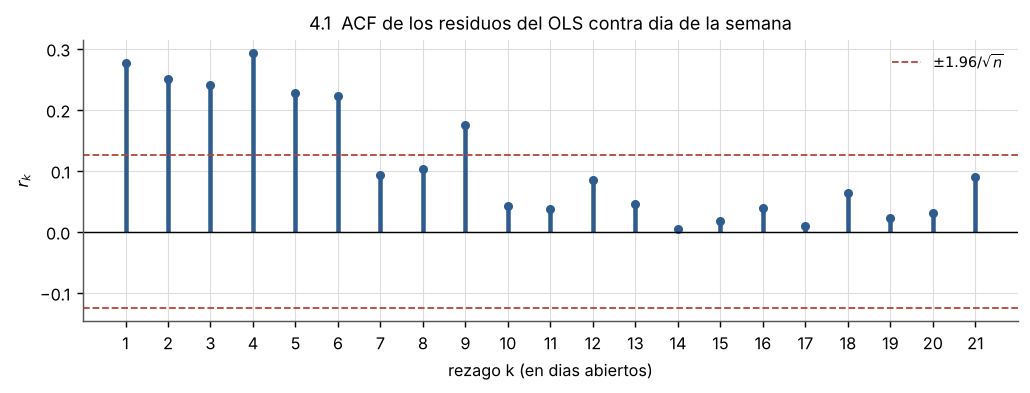
\includegraphics[width=\textwidth]{../figuras/p4_acf_residuos_ols.png}
\caption{ACF de los residuos $e_t$ del OLS contra indicadoras de d\'ia de la
semana. \textbf{Qu\'e muestra:} el pico gigante del rezago~6 desapareci\'o
(baj\'o de \num{0.42} a \num{0.22}) y en su lugar quedaron siete rezagos
fuera de banda, los seis primeros consecutivos y decrecientes.
\textbf{Por qu\'e importa:} esta forma es la de una serie con la media
todav\'ia movi\'endose, no la de un AR(1).}
\end{figure}

\paragraph{{\normalfont\itshape ¿Qu\'e cambi\'o respecto a 3.3?}} Dos cosas.
La estacionalidad se redujo mucho: $r_6$ baj\'o de \num{0.4224} a
\num{0.2224}, as\'i que las indicadoras de d\'ia de la semana se llevaron
cerca de la mitad del pico semanal (no todo, porque el efecto del d\'ia de la
semana es multiplicativo sobre un nivel que cambia, y el OLS lo est\'a
modelando como aditivo y constante). Pero el n\'umero de rezagos fuera de
banda \emph{subi\'o} de seis a siete, y ahora los rezagos \num{1} a~\num{6}
est\'an \emph{todos} fuera: $r_1$ incluso creci\'o, de \num{0.2092} a
\num{0.2759}. Quitar la estacionalidad destap\'o la estructura que estaba
debajo.

\paragraph{{\normalfont\itshape Comparen la forma de esta ACF con las de la
Parte~0: ¿decae como $\phi^k$, como un AR(1), o se parece m\'as a la del
proceso con tendencia?}} \textbf{Se parece mucho m\'as a la del proceso con
tendencia.} Un AR(1) con $\phi \approx \num{0.28}$ (que es lo que sugiere
$r_1$) tendr\'ia $r_2 \approx \num{0.08}$, $r_3 \approx \num{0.02}$ y
pr\'acticamente nada de ah\'i en adelante: la ACF se hunde dentro de las
bandas al segundo o tercer rezago. Lo que se observa es un decaimiento
\emph{mucho m\'as lento}, con seis rezagos consecutivos fuera de banda. Esa
caida lenta es precisamente la pista visual que menciona FPP2 \S8.1 para una
serie \textbf{no estacionaria}: la ACF de una serie estacionaria cae a cero
r\'apido, la de una no estacionaria baja despacio.

\paragraph{{\normalfont\itshape ¿Qu\'e le falta a este modelo?}} Le falta la
\textbf{tendencia}, que es lo que 3.1 mostr\'o y lo que la ACF est\'a
gritando. El OLS contra indicadoras de d\'ia de la semana le asigna a cada
jueves del a\~no el mismo valor ajustado, \gbp\num{36094}, sin importar que
los jueves de febrero vendieran alrededor de \gbp\num{20000} y los de
noviembre m\'as de \gbp\num{55000}. Todos los residuos de la primera mitad
del a\~no quedan negativos y los de la segunda positivos, y residuos vecinos
se parecen entre s\'i por esa raz\'on y no porque haya memoria. Es
exactamente el mecanismo de la tendencia lineal de 0.4. Tambi\'en le falta
permitir que el tama\~no del efecto semanal crezca con el nivel, que es lo
que motiva trabajar en logaritmos en 4.3.

\subsection{4.2 Un AR(1) para la memoria que queda}

Regresando $e_t$ contra $e_{t-1}$ por OLS se obtiene
$\hat\phi = \num{0.2779}$ (con $\hat c = \num{-103.5}$, pr\'acticamente
cero como corresponde a residuos de una regresi\'on con indicadoras
completas).

\begin{figure}[htbp]
\centering
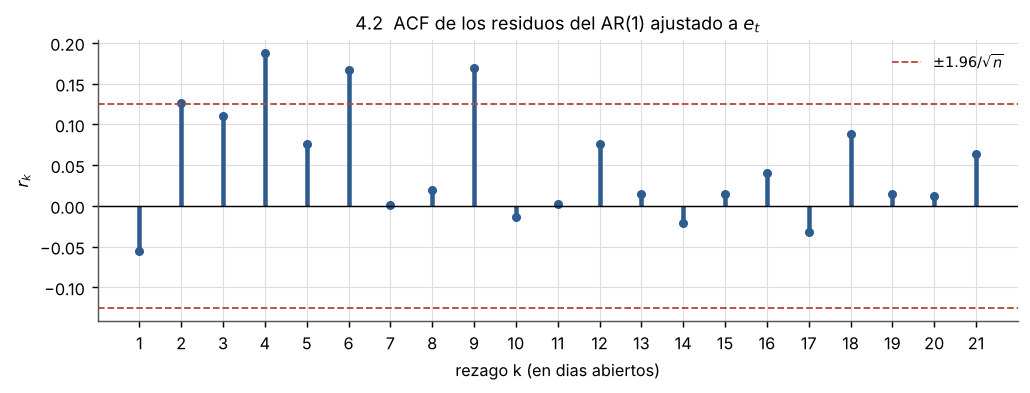
\includegraphics[width=\textwidth]{../figuras/p4_acf_residuos_ar1.png}
\caption{ACF de los residuos $u_t = e_t - \hat c - \hat\phi e_{t-1}$.
\textbf{Qu\'e muestra:} el AR(1) limpi\'o el rezago~1, que ya est\'a dentro
de las bandas, pero dej\'o afuera los rezagos \num{2}, \num{4}, \num{6}
y~\num{9}. \textbf{Por qu\'e importa:} el rezago~6 sigue vivo, y eso es
estacionalidad, que un AR(1) no tiene c\'omo capturar.}
\end{figure}

\begin{table}[htbp]
\centering
\footnotesize
\caption{\textbf{4.2} AR(1) ajustado por OLS a los residuos $e_t$ del inciso 4.1, y Ljung--Box sobre sus residuos $u_t$ (un grado de libertad menos por el $\phi$ estimado).}
\label{tab:p4_ar1}
\begin{tabular}{lr}
\toprule
\textbf{cantidad} & \textbf{valor} \\
\midrule
c & -103.51 \\
phi & 0.2779 \\
desv\_est\_residuos\_u & 11\,901.04 \\
LjungBox Q(6) & 25.0364 \\
LjungBox Q(6) gl & 5.0000 \\
LjungBox Q(6) valor\_p & 0.0001 \\
LjungBox Q(12) & 33.9542 \\
LjungBox Q(12) gl & 11.0000 \\
LjungBox Q(12) valor\_p & 0.0004 \\
\bottomrule
\end{tabular}
\\[0.3em]{\scriptsize \textbf{Qu\'e leer:} $\hat\phi=0.278$ limpia el rezago~1, pero ambas pruebas siguen rechazando: quedan fuera de banda los rezagos 2, 4, 6 y 9. Un AR(1) implica $\rho_6=0.28^6\approx0.0005$, o sea que predice que no hay nada en el rezago 6, y s\'i lo hay.}
\end{table}


\paragraph{{\normalfont\itshape ¿Ya parecen ruido blanco?}} \textbf{No.}
$Q(6) = \num{25.04}$ con \num{5} grados de libertad da $p = \num{1.4e-4}$, y
$Q(12) = \num{33.95}$ con \num{11} grados de libertad da $p = \num{3.7e-4}$
(se descuenta un grado de libertad en cada caso por el $\phi$ estimado,
siguiendo Tsay \S2.4). Ambas rechazan con holgura.

\paragraph{{\normalfont\itshape ¿Qu\'e rezagos siguen fuera de las
bandas?}} Los rezagos \textbf{\num{2}, \num{4}, \num{6} y~\num{9}}. El
\num{1} s\'i qued\'o limpio, que es justo lo que un AR(1) sabe hacer.

\paragraph{{\normalfont\itshape ¿Alcanz\'o un AR(1) para lo que encontraron
en 4.1?}} \textbf{No, y no pod\'ia alcanzar.} El AR(1) tiene un solo
par\'ametro y lo gasta todo en el rezago~1. Pero el problema de 4.1 no era
el rezago~1: era un decaimiento lento que delata una media que se mueve, y
un pico estacional en el rezago~6 que sobrevivi\'o a las indicadoras. Un
AR(1) con $\hat\phi = \num{0.28}$ implica $\rho_6 = \num{0.28}^6 \approx
\num{0.0005}$, o sea que el modelo predice que \emph{no hay} nada en el
rezago~6, mientras los datos muestran que s\'i lo hay. Se necesitan dos
herramientas que el AR(1) no tiene: un t\'ermino \textbf{estacional} que
mire directamente el rezago~6, y una \textbf{diferenciaci\'on} que se
encargue de la media que se mueve. Eso es exactamente la familia SARIMA.

\subsection{4.3 SARIMA}

Siguiendo el enunciado, ambos modelos se ajustan sobre el \textbf{logaritmo}
de la venta diaria, con $s=6$, pas\'andole al estimador el arreglo de valores
y no la serie con fechas.

\paragraph{{\normalfont\itshape ¿Por qu\'e $s=6$ y no~7?}} Porque la serie
que se modela es la de d\'ias \emph{abiertos}, una fila por d\'ia, y la
tienda cierra los s\'abados: entre un jueves y el jueves anterior hay seis
filas, no siete. Esto no es una conjetura sino un hallazgo medido: el
inciso~3.3 verific\'o que el pico de la ACF est\'a en $k=6$ y que esos seis
d\'ias abiertos corresponden a siete d\'ias calendario. Si se usara $s=7$ el
t\'ermino estacional apuntar\'ia al \emph{viernes} anterior cuando el d\'ia
es jueves, y el modelo buscar\'ia la estacionalidad donde no est\'a.

\paragraph{{\normalfont\itshape ¿Cu\'ando se rompe ese supuesto en estos
datos?}} En las semanas con feriado. El supuesto de ``seis filas $=$ una
semana'' vale solo si cada semana aporta exactamente seis d\'ias abiertos, y
eso falla en las \num{11} semanas con feriado bancario: en la semana de
Pascua, por ejemplo, la tienda abri\'o cuatro d\'ias, as\'i que el rezago~6
apunta a un d\'ia de la semana equivocado. La verificaci\'on emp\'irica de
3.3 lo cuantifica: la distancia calendario del rezago~6 es de siete d\'ias en
la mediana, pero llega a \num{18} en el peor caso. Es una aproximaci\'on,
buena la mayor parte del a\~no y mala alrededor de los feriados, y es parte
del precio de modelar d\'ias abiertos como si fueran una rejilla regular.

\paragraph{{\normalfont\itshape ¿Por qu\'e el logaritmo?}} Por tres razones
que apuntan en la misma direcci\'on. Primero, la variabilidad de la serie
crece con su nivel: en los meses planos las oscilaciones diarias son de unos
pocos miles de libras y en noviembre son de decenas de miles. El logaritmo
estabiliza esa varianza, que es justo el caso que FPP2 \S3.2 describe para
una transformaci\'on. Segundo, el efecto del d\'ia de la semana es
\emph{multiplicativo} (3.2 lo midi\'o como un \'indice, no como un monto
fijo), y en logaritmos un efecto multiplicativo se vuelve aditivo, que es lo
que un modelo lineal sabe manejar. Tercero, el logaritmo garantiza que el
pron\'ostico al deshacer la transformaci\'on sea positivo. Como se ajust\'o
en logaritmos, para volver a libras se aplica \texttt{exp()} al pron\'ostico,
sin correcci\'on de sesgo, tal como indica el enunciado; con eso el
pron\'ostico es la mediana condicional y no la media.

\begin{table}[htbp]
\centering
\footnotesize
\caption{\textbf{4.3} Los dos modelos SARIMA ajustados sobre $\log$(venta diaria) con $s=6$, por m\'axima verosimilitud exacta (filtro de Kalman).}
\label{tab:p4_sarima}
\begin{tabular}{lcccccccc}
\toprule
\textbf{modelo} & \textbf{$\hat\phi$} & \textbf{$\hat\Phi$} & \textbf{$\hat\theta$} & \textbf{$\hat\Theta$} & \textbf{$\hat\mu$} & \textbf{$\hat\sigma^2$} & \textbf{log-verosim.} & \textbf{conv.} \\
\midrule
S1  SARIMA(1,0,0)(1,0,0)\_6 con con & 0.1216 & 0.5296 & --- & --- & 10.1480 & 0.21677 & -161.344 & s\'i \\
S2  SARIMA(0,1,1)(0,1,1)\_6 sin con & --- & --- & -0.9179 & -0.6612 & --- & 0.21364 & -157.188 & s\'i \\
\bottomrule
\end{tabular}
\\[0.3em]{\scriptsize \textbf{Qu\'e leer:} en S1 el t\'ermino estacional ($\hat\Phi=0.53$) pesa mucho m\'as que el regular ($\hat\phi=0.12$), confirmando que el rezago 6 es el que importa. Ambos modelos convergieron ya con el \texttt{maxiter} por omisi\'on; con \texttt{maxiter}=500 los par\'ametros son id\'enticos a cuatro decimales.}
\end{table}


\paragraph{Convergencia.} Se verific\'o \texttt{mle\_retvals['converged']}
en ambos modelos. Los dos convergieron ya con el \texttt{maxiter} por
omisi\'on, as\'i que no hizo falta subirlo; por control se repiti\'o el
ajuste con \texttt{maxiter=500} y los par\'ametros resultaron id\'enticos
hasta la cuarta cifra decimal y la log-verosimilitud coincide en los tres
decimales reportados. En la Parte~5, donde ambos modelos se reajustan en
cada origen m\'ovil, se us\'o la configuraci\'on que convergi\'o aqu\'i y se
verific\'o la convergencia en cada origen: S1 y S2 convergieron en los
\num{22} or\'igenes de entrenamiento y en los \num{10} de prueba.

Los par\'ametros estimados son coherentes con el diagn\'ostico de 4.1 y 4.2.
En S1 el t\'ermino estacional domina ($\hat\Phi = \num{0.5296}$) sobre el
regular ($\hat\phi = \num{0.1216}$): el modelo confirma que el rezago~6
importa mucho m\'as que el rezago~1. En S2 ambos coeficientes MA son grandes
y negativos ($\hat\theta = \num{-0.9179}$,
$\hat\Theta = \num{-0.6612}$), que es la firma t\'ipica del modelo de
aerol\'inea cuando las diferencias han sobre-diferenciado un poco la serie.

\subsection{4.4 Diagn\'ostico}

\begin{table}[htbp]
\centering
\footnotesize
\caption{\textbf{4.4} Ljung--Box sobre los residuos. En S2 se descartan los primeros 7 residuos, que son artefactos del arranque de las diferencias $(1-B)(1-B^6)$. Los grados de libertad bajan a $m-2$ en ambos modelos.}
\label{tab:p4_diagnostico}
\begin{tabular}{ccccccc}
\toprule
\textbf{modelo} & \textbf{$m$} & \textbf{$n$ residuos} & \textbf{$Q(m)$} & \textbf{gl} & \textbf{valor-$p$} & \textbf{ruido blanco} \\
\midrule
S1 & 6 & 245 & 9.72 & 4 & 0.0454 & no \\
S1 & 12 & 245 & 23.36 & 10 & 0.0095 & no \\
S2 & 6 & 231 & 4.31 & 4 & 0.3655 & \textbf{s\'i} \\
S2 & 12 & 231 & 11.76 & 10 & 0.3015 & \textbf{s\'i} \\
\bottomrule
\end{tabular}
\\[0.3em]{\scriptsize \textbf{Qu\'e leer:} S2 es el \'unico que deja residuos de ruido blanco. S1 es estacionario y supone una media fija que no existe, as\'i que la tendencia de agosto en adelante se le queda en los residuos. Este resultado anticipa correctamente qui\'en gana en la Parte~5.}
\end{table}


En S2 se descartaron los primeros \num{7} residuos: las diferencias
$(1-B)(1-B^6)$ se comen $d + Ds = 1 + 6 = 7$ observaciones y esos residuos
son artefactos del arranque, no informaci\'on sobre el modelo. En ambos
modelos los grados de libertad bajan a $m-2$ porque cada uno estima dos
par\'ametros en la parte ARMA.

\paragraph{{\normalfont\itshape ¿Cu\'al modelo deja residuos de ruido
blanco?}} \textbf{S2, y solo S2.}

Para \textbf{S1}, $Q(6) = \num{9.72}$ con \num{4} grados de libertad da
$p = \num{0.045}$ y $Q(12) = \num{23.36}$ con \num{10} grados de libertad da
$p = \num{0.0095}$. Ambas rechazan al \SI{5}{\percent}, aunque $Q(6)$ lo hace
por poco. Este es el \'unico caso de toda la tarea donde la elecci\'on de~$m$
cambia la contundencia de la conclusi\'on: con $m=6$ el valor-$p$ queda
justo en el filo y con $m=12$ el rechazo es claro. Como los dos apuntan en la
misma direcci\'on, la conclusi\'on es que S1 \textbf{no} deja ruido blanco.

Para \textbf{S2}, $Q(6) = \num{4.31}$ ($p=\num{0.365}$) y
$Q(12) = \num{11.76}$ ($p=\num{0.301}$). Ninguna se acerca a rechazar: los
residuos de S2 son indistinguibles de ruido blanco.

La diferencia tiene una explicaci\'on clara y es la misma que se viene
arrastrando desde 4.1. S1 es un modelo \textbf{estacionario}: supone que la
serie oscila alrededor de una media fija, y esa suposici\'on es falsa aqu\'i
porque el nivel sube a partir de agosto. Esa tendencia no modelada se queda
en los residuos y aparece como autocorrelaci\'on. S2, en cambio,
\emph{diferencia} la serie en los dos sentidos, $(1-B)$ y $(1-B^6)$, y la
diferenciaci\'on es precisamente el truco para series cuya media se mueve: le
quita a la serie la obligaci\'on de volver a un nivel fijo. Por eso S2 puede
seguir la subida y S1 no.

\subsection{4.5 {\normalfont\itshape ¿Hacia d\'onde van los pron\'osticos?}}

\paragraph{S1: hacia la media, y se queda ah\'i.} S1 es estacionario, y un
proceso estacionario olvida. Es el mismo argumento del AR(1) de la Parte~0
con $|\phi|<1$: la influencia del \'ultimo valor observado se multiplica por
$\phi$ (y por $\Phi$ en la parte estacional) en cada paso hacia adelante,
as\'i que se desvanece geom\'etricamente, y el pron\'ostico converge a la
media incondicional del modelo. Los n\'umeros lo muestran limpiamente: a un
paso pronostica \gbp\num{29402}, a \num{30} pasos \gbp\num{26124}, y a
\num{120} pasos \gbp\num{25539}, que es exactamente
$\exp(\hat\mu) = \gbp\num{25539}$. De ah\'i ya no se mueve. Para horizontes
largos, S1 no dice nada m\'as interesante que ``la venta t\'ipica''.

\paragraph{S2: se va, sin l\'imite.} S2 no es estacionario, y por el lado
contrario: con $d=1$, la serie en niveles es una caminata aleatoria (con
estructura MA encima), y una caminata aleatoria nunca olvida. El
pron\'ostico no tiene una media a la cual regresar, as\'i que arrastra
indefinidamente el nivel y la pendiente que ten\'ia al final de los datos.
Los n\'umeros: \gbp\num{29118} a un paso, \gbp\num{61148} a \num{30} pasos y
\gbp\num{174338} a \num{120} pasos, creciendo sin freno. Como los datos
terminan en plena subida navide\~na, S2 extrapola esa subida para siempre, lo
cual es razonable a unos pocos d\'ias y absurdo a seis meses. Adem\'as sus
intervalos de predicci\'on se abren indefinidamente, igual que la
$\operatorname{Var}(Y_t) = t\sigma^2$ de la caminata aleatoria del
inciso~0.1.

\textbf{La moraleja pr\'actica} es que la ventaja de S2 en 4.4 y la que se
ver\'a en la Parte~5 es una ventaja \emph{de horizonte corto}. Es el modelo
correcto para pronosticar la pr\'oxima semana porque puede seguir el nivel
que se mueve; ser\'ia el modelo equivocado para pronosticar el pr\'oximo
a\~no.

% ===========================================================================
\section{Parte 5: Pron\'ostico y fuga}
% ===========================================================================

\subsection{5.1 Los seis modelos}

Adem\'as de S1 y S2 se implementaron cuatro modelos m\'as:
\begin{description}[leftmargin=2.6em,style=nextline,nosep]
  \item[B1] La media hist\'orica de los d\'ias abiertos. Un n\'umero
  constante.
  \item[B2] Naive estacional: el valor del mismo d\'ia de la semana abierto
  m\'as reciente. Es el pron\'ostico de una caminata aleatoria estacional.
  \item[M1] OLS con una tendencia lineal en~$t$ e indicadoras de d\'ia de la
  semana.
  \item[M2] OLS con indicadoras de d\'ia de la semana y los rezagos
  $y_{t-7}$ e $y_{t-14}$. Cuando alguno cae en d\'ia cerrado se usa el mismo
  d\'ia de la semana abierto m\'as reciente; las filas que se quedan sin
  rezago al inicio no se usan para ajustar.
\end{description}

\paragraph{{\normalfont\itshape ¿Por qu\'e M2 puede usar $y_{t-7}$ para
pronosticar cualquiera de los siete d\'ias siguientes, pero no podr\'ia usar
$y_{t-1}$?}} Porque el origen es un domingo y el objetivo m\'as lejano es el
domingo siguiente, siete d\'ias calendario despu\'es. Para ese objetivo,
$y_{t-7}$ es la venta del \emph{domingo origen}, que ya est\'a observada
(el enunciado lo dice expl\'icitamente: la venta del origen ya forma parte de
lo observado). Para cualquier objetivo m\'as cercano, $y_{t-7}$ cae a\'un
antes, as\'i que con m\'as raz\'on ya se conoce. Es decir, el rezago~7 nunca
cruza la frontera del presente.

Con $y_{t-1}$ ser\'ia distinto. Para pronosticar el martes habr\'ia que
conocer la venta del lunes, que todav\'ia no ha ocurrido: est\'a del lado del
futuro. Usarla ser\'ia darle al modelo informaci\'on que no tendr\'ia un
usuario real el domingo por la noche, que es precisamente la definici\'on de
fuga. El rezago~7 funciona porque es, justamente, la distancia del ciclo que
separa al origen de su objetivo m\'as lejano.

\paragraph{{\normalfont\itshape ¿C\'omo le hace S1 para usar el rezago~1 de
todas formas?}} Pronosticando de forma \emph{recursiva}. S1 s\'i usa el
rezago~1, pero para el horizonte~1 usa el valor \emph{observado} del origen,
y para el horizonte~2 en adelante sustituye el valor que no conoce por su
propio pron\'ostico del paso anterior. No hace trampa: nunca mira un dato que
no tiene, solo encadena sus propias predicciones. El precio es que el error
se acumula, y por eso la calidad de los modelos recursivos se degrada
conforme crece el horizonte.

\subsection{5.2--5.3 Los tres estimados del error}

\begin{table}[htbp]
\centering
\footnotesize
\caption{\textbf{5.2--5.3} MAE y RMSE en libras de los seis modelos, estimados de tres formas: (a) validaci\'on cruzada aleatoria de 5 \emph{folds} sobre el entrenamiento con 10 semillas (media $\pm$ desviaci\'on est\'andar entre semillas), (b) origen m\'ovil semanal dentro del entrenamiento con 22 or\'igenes de mayo a septiembre, (c) origen m\'ovil semanal en la prueba con 10 or\'igenes, 58 d\'ias evaluados.}
\label{tab:p5_resultados}
\begin{tabular}{lrrrrrr}
\toprule
\textbf{modelo} & \textbf{MAE (a)} & \textbf{RMSE (a)} & \textbf{MAE (b)} & \textbf{RMSE (b)} & \textbf{\textbf{MAE (c)}} & \textbf{\textbf{RMSE (c)}} \\
\midrule
\textbf{B1} & 10\,565 \tiny$\pm$67 & 14\,654 & 10\,506 & 15\,254 & 23\,446 & 28\,179 \\
\textbf{B2} & --- & --- & 11\,634 & 15\,949 & 14\,655 & 18\,957 \\
\textbf{M1} & 9\,361 \tiny$\pm$86 & 12\,879 & 9\,997 & 14\,147 & 15\,759 & 20\,955 \\
\textbf{M2} & 8\,522 \tiny$\pm$106 & 12\,007 & 9\,480 & 13\,675 & 15\,648 & 20\,393 \\
\textbf{S1} & --- & --- & 9\,854 & 14\,036 & 17\,243 & 21\,657 \\
\textbf{S2} & --- & --- & 10\,304 & 14\,325 & 12\,817 & 16\,217 \\
\bottomrule
\end{tabular}
\\[0.3em]{\scriptsize \textbf{Qu\'e leer:} (c) es la columna honesta y S2 gana por los dos criterios. (a) no aplica a B2, S1 y S2 porque los tres dependen del orden del tiempo. Y los tres estimados de adentro se quedan cortos: para M2, (b) subestima el error real en un 39\,\%.}
\end{table}


\begin{figure}[htbp]
\centering
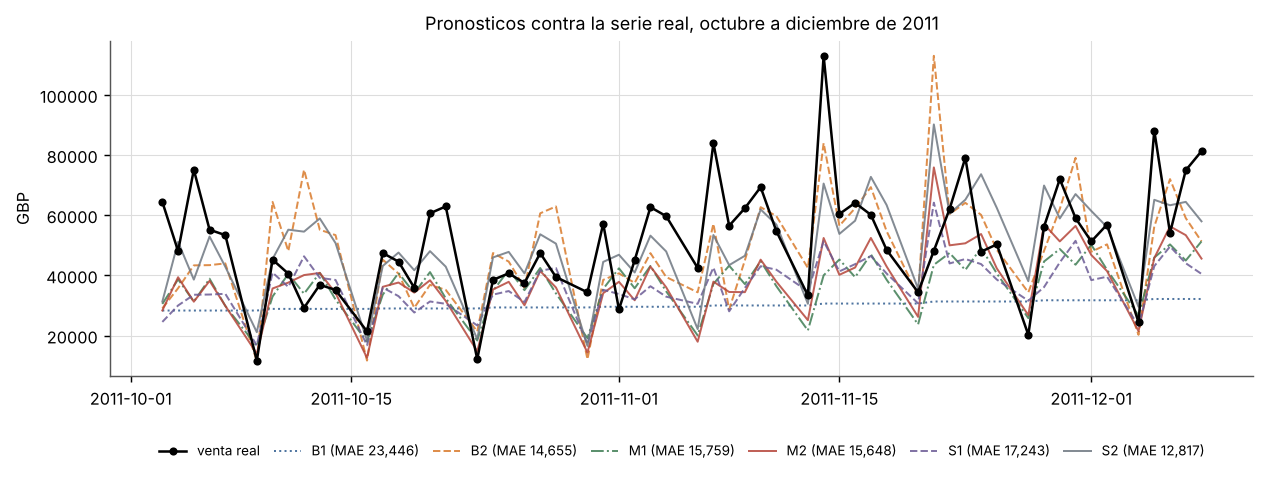
\includegraphics[width=\textwidth]{../figuras/p5_prueba.png}
\caption{Pron\'osticos de los seis modelos contra la serie real en el
per\'iodo de prueba, con origen m\'ovil semanal. \textbf{Qu\'e muestra:} la
l\'inea negra es la venta real y las dem\'as son los pron\'osticos.
\textbf{Por qu\'e importa:} se ve que \emph{todos} los modelos van por debajo
de la realidad durante casi todo el per\'iodo, porque todos fueron
entrenados con datos de un nivel m\'as bajo. B1, la l\'inea punteada
horizontal cerca de \gbp\num{30000}, ni siquiera intenta seguir el
movimiento. S2 es el que m\'as se acerca al nivel alto de noviembre.}
\end{figure}

\paragraph{{\normalfont\itshape ¿Por qu\'e no tiene sentido (a) para B2, S1
y S2?}} Porque la validaci\'on cruzada aleatoria \emph{baraja las filas}, y
esos tres modelos est\'an definidos por el orden del tiempo. B2 necesita
saber cu\'al es el d\'ia abierto m\'as reciente del mismo d\'ia de la
semana; si el conjunto de entrenamiento es un subconjunto aleatorio de d\'ias,
``el m\'as reciente'' deja de estar bien definido y, lo que es peor, puede
caer \emph{despu\'es} del d\'ia que se quiere predecir. S1 y S2 necesitan una
serie contigua: el filtro de Kalman recorre las observaciones una tras otra
y las diferencias $(1-B)(1-B^6)$ no significan nada si faltan filas al azar
en medio. B1, M1 y M2, en cambio, son modelos de \emph{fila}: su predicci\'on
para un d\'ia depende solo de las variables de esa fila, as\'i que barajar no
los rompe mec\'anicamente. (Que no los rompa mec\'anicamente no quiere decir
que el resultado sea v\'alido; de eso trata 5.5.)

\paragraph{{\normalfont\itshape ¿Cu\'al de (a) y (b) se acerca m\'as a (c)?
¿Alguna se acerca de verdad?}} \textbf{(b) se acerca m\'as, pero ninguna se
acerca de verdad.} Comparando sobre los modelos que admiten las tres
estimaciones, M1 y M2: en (a) el MAE es de \gbp\num{9361} y \gbp\num{8522},
en (b) sube a \gbp\num{9997} y \gbp\num{9480}, y en (c) salta a
\gbp\num{15759} y \gbp\num{15648}. El origen m\'ovil es un poco m\'as
pesimista que la validaci\'on cruzada, que es lo correcto, pero ambos se
quedan cort\'isimos: (b) subestima el error de prueba en un
\SI{39}{\percent} para M2, y (a) en un \SI{46}{\percent}. Para B1 la
distancia es a\'un m\'as brutal: \gbp\num{10506} en (b) contra
\gbp\num{23446} en (c), m\'as del doble. Las causas se separan en 5.5.

\paragraph{5.3 {\normalfont\itshape ¿Qu\'e modelo gana en prueba?}}
\textbf{S2}, y gana por los dos criterios: MAE de \gbp\num{12817} (el
siguiente es B2 con \gbp\num{14655}) y RMSE de \gbp\num{16217} (el siguiente
es B2 con \gbp\num{18957}). El orden completo por MAE es S2 $<$ B2 $<$ M2
$<$ M1 $<$ S1 $<$ B1.

\emph{Por qu\'e gana.} La respuesta est\'a en el inciso~4.4 y en la figura.
El per\'iodo de prueba cae \'integramente sobre la subida navide\~na, as\'i
que el problema dominante no es capturar el patr\'on semanal (eso lo hacen
casi todos) sino \textbf{seguir un nivel que sube}. S2 es el \'unico modelo
del conjunto que diferencia la serie, y diferenciar es exactamente lo que
libera al pron\'ostico de tener que volver a una media fija: arrastra el
nivel reci\'en observado hacia adelante. Esto conecta directamente con 4.4:
S2 fue tambi\'en el \'unico cuyos residuos pasaron Ljung--Box, y pasaron
porque no le quedaba tendencia sin modelar. El diagn\'ostico de residuos
anticip\'o correctamente qui\'en ganar\'ia en prueba.

El reverso lo confirma: \textbf{B1 es el peor con diferencia}
(\gbp\num{23446}, casi el doble que S2) justamente porque es el modelo m\'as
anclado a la media hist\'orica, un n\'umero constante calculado sobre un
a\~no cuyo nivel t\'ipico ya no aplica. Y \textbf{S1 queda quinto}
(\gbp\num{17243}), peor que modelos mucho m\'as simples, por la misma
raz\'on: es estacionario y jala el pron\'ostico de vuelta hacia
$\exp(\hat\mu) \approx \gbp\num{25539}$ cuando la realidad anda por encima de
\gbp\num{60000}. Es notable que \textbf{B2, un naive estacional sin ning\'un
par\'ametro}, quede segundo y le gane a los dos modelos de regresi\'on y a
S1: cuando el nivel se mueve r\'apido, copiar el valor m\'as reciente del
mismo d\'ia de la semana es una estrategia dif\'icil de superar.

\subsection{5.4 La trampa}

Un compa\~nero propone agregar a M2 la media m\'ovil centrada de siete d\'ias
de la Parte~3 como predictor, porque ``resume la tendencia''. Se hizo.

\begin{table}[htbp]
\centering
\footnotesize
\caption{\textbf{5.4} La trampa: M2 con la media m\'ovil \emph{centrada} de 7 d\'ias agregada como predictor.}
\label{tab:p5_trampa}
\begin{tabular}{lrrrrrr}
\toprule
\textbf{modelo} & \textbf{MAE (a)} & \textbf{RMSE (a)} & \textbf{MAE (b)} & \textbf{RMSE (b)} & \textbf{MAE (c)} & \textbf{RMSE (c)} \\
\midrule
\textbf{M2} & 8\,522 & 12\,007 & 9\,480 & 13\,675 & --- & --- \\
\textbf{M2 + MA7 (ilegal)} & 7\,683 & 10\,374 & 8\,585 & 11\,640 & \textbf{imposible} & --- \\
\bottomrule
\end{tabular}
\\[0.3em]{\scriptsize \textbf{Qu\'e leer:} el predictor ilegal mejora el MAE un 9.8\,\% en (a) y un 9.4\,\% en (b), y ninguna de las dos validaciones protesta. La \'unica se\~nal de alarma es que (c) no se puede calcular: $\mathrm{MA}_t$ necesita $y_{t+1}$, $y_{t+2}$, $y_{t+3}$ y adem\'as contiene $y_t/7$, que es la propia respuesta.}
\end{table}


\begin{figure}[htbp]
\centering
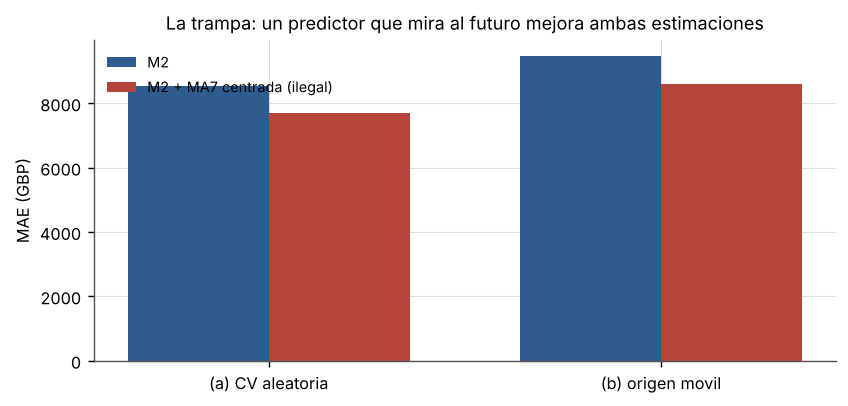
\includegraphics[width=0.68\textwidth]{../figuras/p5_trampa.png}
\caption{MAE de M2 con y sin la media m\'ovil centrada como predictor.
\textbf{Qu\'e muestra:} el predictor ilegal baja el error en las dos formas
de estimarlo. \textbf{Por qu\'e importa:} ninguna de las dos validaciones
emite se\~nal de alarma. Un equipo que solo mirara estos n\'umeros
concluir\'ia que acaba de mejorar su modelo.}
\end{figure}

\paragraph{{\normalfont\itshape ¿Se ve mejor?}} \textbf{S\'i, se ve claramente
mejor, y ese es el problema.} En la validaci\'on cruzada aleatoria el MAE
baja de \gbp\num{8522} a \gbp\num{7683}, una mejora del
\SI{9.8}{\percent}. En el origen m\'ovil dentro del entrenamiento baja de
\gbp\num{9480} a \gbp\num{8585}, una mejora del \SI{9.4}{\percent}. El RMSE
mejora a\'un m\'as, un \SI{14}{\percent} en ambos casos. Son mejoras del
tama\~no que uno celebrar\'ia en una reuni\'on.

\paragraph{{\normalfont\itshape ¿Por qu\'e ese predictor es ilegal?}} Porque
\textbf{mira al futuro}. La media m\'ovil centrada de siete d\'ias en el
d\'ia~$t$ es
\[
\mathrm{MA}_t = \frac{1}{7}\sum_{j=-3}^{3} y_{t+j}
= \frac{y_{t-3}+y_{t-2}+y_{t-1}+y_t+y_{t+1}+y_{t+2}+y_{t+3}}{7}.
\]
Tres de los siete sumandos, $y_{t+1}$, $y_{t+2}$ e $y_{t+3}$, son d\'ias
posteriores a~$t$. Y el cuarto, $y_t$, \emph{es la propia variable que se
quiere pronosticar}: el predictor contiene $1/7$ de la respuesta. Nadie
parado el domingo por la noche puede calcular el $\mathrm{MA}$ centrado del
mi\'ercoles siguiente, porque para eso necesitar\'ia las ventas del jueves,
viernes y s\'abado de esa semana. El modelo no est\'a pronosticando: est\'a
leyendo una versi\'on suavizada de la respuesta.

\paragraph{{\normalfont\itshape ¿Por qu\'e el origen m\'ovil \emph{no} lo
detecta si la media m\'ovil se calcula una sola vez sobre toda la serie?}}
Porque el origen m\'ovil solo controla \emph{qu\'e filas} entran al ajuste,
no \emph{c\'omo se construyeron las columnas}. La fuga ocurre antes, en el
momento de calcular la columna \texttt{ma7} sobre la serie completa. Para
cuando el origen m\'ovil corta en el domingo y dice ``entrena con esto,
predice aquello'', el valor de \texttt{ma7} de cada fila del futuro
\emph{ya trae dentro} la informaci\'on de sus d\'ias vecinos. El corte
temporal est\'a bien hecho; la contaminaci\'on viaja \emph{dentro} de una
columna que el corte no toca.

Esta es la lecci\'on general y es la m\'as importante de la Parte~5: una
validaci\'on, por rigurosa que sea, solo protege contra la fuga que ocurre
\emph{despu\'es} del punto donde ella act\'ua. La regla pr\'actica que se
deriva es que toda transformaci\'on que use datos de varias filas (medias
m\'oviles, normalizaciones, imputaciones, codificaciones por promedio de la
variable objetivo, selecci\'on de variables) debe recalcularse \emph{dentro}
de cada pliegue, nunca una sola vez sobre el conjunto completo. Si la columna
se calcula una vez, el origen m\'ovil se vuelve teatro.

\paragraph{{\normalfont\itshape ¿Por qu\'e no pueden calcular (c) sin hacer
trampa?}} Porque para pronosticar el d\'ia~$t$ del per\'iodo de prueba
har\'ia falta $\mathrm{MA}_t$, y $\mathrm{MA}_t$ necesita $y_{t+1}$,
$y_{t+2}$ e $y_{t+3}$, que son d\'ias del per\'iodo de prueba a\'un no
observados en el momento del pron\'ostico. La \'unica forma de producir un
n\'umero para (c) ser\'ia ir a buscar esos valores al conjunto de prueba, que
es precisamente lo que el conjunto de prueba existe para impedir. Por eso la
celda correspondiente de la tabla est\'a vac\'ia y debe quedarse vac\'ia:
\textbf{la imposibilidad de calcular (c) es el s\'intoma de que el predictor
no sirve}, y es la \'unica de las tres validaciones que detecta el
problema. Un predictor que no se puede calcular en producci\'on no se puede
usar en producci\'on, por bien que luzca en el laboratorio.

\subsection{5.5 Por qu\'e todo lo estimado adentro se queda corto}

Todas las estimaciones hechas dentro del entrenamiento se quedan cortas
frente al error de prueba. Hay \textbf{dos causas distintas} y conviene
separarlas porque tienen remedios opuestos.

\paragraph{Causa 1: c\'omo se partieron los datos.} La validaci\'on cruzada
aleatoria le permite al modelo entrenar con d\'ias \emph{posteriores} a los
que predice. Como la serie tiene tendencia y autocorrelaci\'on, un d\'ia de
entrenamiento del 15 de septiembre le dice muchas cosas sobre un d\'ia de
prueba del 14 de septiembre que no se sabr\'ian de antemano. Adem\'as el
horizonte efectivo de la validaci\'on cruzada es de cero d\'ias, mientras que
el horizonte real va de uno a siete. Esto infla el optimismo de (a).

\textbf{Esta causa s\'i se arregla con una mejor validaci\'on}, y de hecho se
ve arreglada en la tabla: al pasar de (a) a (b) el MAE de M2 sube de
\gbp\num{8522} a \gbp\num{9480} y el de M1 de \gbp\num{9361} a
\gbp\num{9997}. Es decir, el origen m\'ovil recupera alrededor de un
\SI{10}{\percent} de pesimismo que la validaci\'on cruzada aleatoria
escond\'ia. Esa diferencia es la medida limpia del sesgo introducido por
partir mal.

\paragraph{Causa 2: la serie cambi\'o.} Pero incluso (b), que est\'a bien
construida, se queda a un \SI{39}{\percent} del error real. Lo que falta no
es un defecto del m\'etodo de validaci\'on sino un hecho del mundo: entre
mayo y septiembre la serie oscilaba alrededor de \gbp\num{20000} a
\gbp\num{30000} diarios, y en noviembre and\'a por encima de
\gbp\num{55000}. El per\'iodo de prueba simplemente \emph{no se parece} al
per\'iodo de entrenamiento. Ninguna forma de partir los datos de mayo a
septiembre puede revelar qu\'e tan dif\'icil es noviembre, porque noviembre
no est\'a ah\'i dentro.

\textbf{Esta causa no se arregla con mejor validaci\'on.} Se puede
reconocer, se puede acotar (por ejemplo reservando siempre el tramo final
como prueba, que es lo que hace el enunciado), se puede mitigar eligiendo
modelos que se adapten r\'apido al nivel reciente, como S2, pero no se puede
estimar desde adentro. Es la diferencia entre varianza de muestreo y cambio
estructural.

\paragraph{{\normalfont\itshape Con un solo a\~no de datos, ¿se puede
estimar la estacionalidad anual?}} \textbf{No.} Para estimar un efecto
estacional de per\'iodo anual hay que observar varios ciclos: con uno solo,
el ``efecto noviembre'' y ``lo que pas\'o en noviembre de 2011'' son
exactamente el mismo n\'umero, y no hay forma de separar el patr\'on que se
repite todos los a\~nos del evento particular de ese a\~no. Formalmente, se
tendr\'ia una observaci\'on por nivel del factor estacional: el par\'ametro
no est\'a identificado y su error est\'andar no se puede estimar.

Esto tiene una consecuencia incomoda y conviene ser expl\'icito: la subida
de noviembre que se observa en estos datos es casi con certeza estacionalidad
navide\~na, pero \textbf{con este archivo no se puede demostrar}. Podr\'ia ser
crecimiento del negocio, una campa\~na de marketing o un cliente mayorista
grande que entr\'o. Los tres se ver\'ian igual. Y por eso ninguno de los
modelos de esta tarea tiene un t\'ermino estacional anual: no se puede
ajustar lo que no se puede identificar. Para capturarlo har\'ian falta al
menos tres o cuatro a\~nos, idealmente m\'as, y aun entonces los feriados
m\'oviles del inciso~2.2 complicar\'ian el asunto.

% ===========================================================================
\section{Parte 6: Detr\'as de la serie hay clientes}
% ===========================================================================

\subsection{6.1 Construcci\'on de R, F y M}

\begin{table}[htbp]
\centering
\footnotesize
\caption{\textbf{6.1--6.5} Resumen del an\'alisis RFM.}
\label{tab:p6_resumen}
\begin{tabular}{lr}
\toprule
\textbf{concepto} & \textbf{valor} \\
\midrule
clientes con transaccion antes del 1-oct & 3658.0 \\
clientes con M <= 0 & 54.0 \\
valores distintos de F & 48.0 \\
compraron en la ventana & 1845.0 \\
tasa base de compra & 0.5044 \\
campeones & 783.0 \\
clientes nuevos en la ventana & 723.0 \\
venta de la ventana (GBP, clientes con ID) & 2432839.69 \\
AUC R (signo invertido) & 0.6764 \\
AUC F (crudo) & 0.721 \\
AUC M (crudo) & 0.7093 \\
AUC suma de los tres puntajes & 0.7352 \\
\bottomrule
\end{tabular}
\\[0.3em]{\scriptsize \textbf{Qu\'e leer:} todo se calcula con transacciones anteriores al 1 de octubre; la ventana del 1 de octubre al 8 de diciembre solo se usa para definir la variable a predecir.}
\end{table}


Usando solo las transacciones anteriores al 1 de octubre de 2011, y solo las
filas limpias con \texttt{CustomerID}, hay \textbf{\num{3658} clientes}.

\paragraph{{\normalfont\itshape ¿Cu\'antos tienen $M \le 0$ y qu\'e hacen con
ellos?}} Son \textbf{\num{54} clientes}, el \SI{1.48}{\percent}, y son
clientes que devolvieron m\'as de lo que compraron: sus cancelaciones superan
sus ventas. Hay adem\'as \num{43} clientes con $F=0$, cuya \'unica actividad
antes de octubre fueron cancelaciones.

\textbf{Se conservan}, por dos razones. La primera es que el propio enunciado
pide incluirlos en el desempate aleatorio de 6.2. La segunda, m\'as de
fondo, es que son informaci\'on leg\'itima y no errores: un cliente con monto
neto negativo es un cliente real con un comportamiento real, y adem\'as es
justamente el tipo de cliente sobre el que uno querr\'ia que el an\'alisis
dijera algo. Al puntuarlos por quintiles caen autom\'aticamente en el
puntaje~1 de~M, que es donde corresponde. Borrarlos hubiera sido m\'as
c\'omodo, pero habr\'ia escondido un \SI{1.5}{\percent} de la base de
clientes sin ninguna justificaci\'on sustantiva. Lo que s\'i se verific\'o es
que son pocos: si fueran el \SI{20}{\percent} har\'ia falta repensar la
definici\'on de~M.

\paragraph{{\normalfont\itshape ¿Por qu\'e es importante no usar nada
posterior al 1 de octubre?}} Porque la variable que se quiere explicar,
\texttt{compra}$_i$, est\'a definida sobre la ventana del 1 de octubre al 8
de diciembre. Si R, F o M se calcularan con datos de esa ventana, el
clasificador tendr\'ia dentro la respuesta y los AUC del inciso~6.3 ser\'ian
ficci\'on: la recencia medida al 8 de diciembre ser\'ia peque\~na justamente
para los clientes que compraron en la ventana, que es lo que se pretende
predecir. Es \textbf{exactamente la misma fuga} del inciso~5.4, con otro
disfraz. All\'a el predictor contaminado era una media m\'ovil centrada;
aqu\'i ser\'ia una recencia calculada demasiado tarde. La disciplina es la
misma: la frontera entre lo observado y lo que se quiere predecir se fija una
vez y no se cruza ni para construir variables.

\subsection{6.2 Puntajes por quintiles}

Se asignaron puntajes de 1 a 5 por quintiles, con 5 como el mejor en las
tres dimensiones (en recencia, 5 es el m\'as reciente, as\'i que las
etiquetas van al rev\'es porque menos d\'ias es mejor). Para el desempate se
sigui\'o el procedimiento exacto del enunciado: todos los clientes de 6.1,
incluidos los de $M \le 0$, ordenados por \texttt{CustomerID} ascendente,
barajados con \texttt{numpy.random.default\_rng(2026).permutation} y
puntuados con \texttt{pd.qcut(F.rank(method='first'), 5)}.

\paragraph{{\normalfont\itshape Van a tener problemas con F. ¿Por qu\'e?}}
Porque \textbf{F es demasiado discreta para partirse en quintiles}. Toma
solo \num{48} valores distintos entre \num{3658} clientes, y est\'a
brutalmente concentrada en los primeros: \num{1444} clientes tienen $F=1$,
\num{693} tienen $F=2$, \num{441} tienen $F=3$. Ese primer grupo, por s\'i
solo, es el \SI{39}{\percent} de la base, casi dos quintiles enteros.

No existe ning\'un corte que parta a los clientes en cinco grupos del
\SI{20}{\percent} cada uno, porque los cortes naturales caen \emph{dentro} de
un empate masivo. El resultado se ve en los rangos efectivos de cada
puntaje: los clientes con $F=1$ terminan repartidos entre los puntajes
\num{1}, \num{2} y~\num{3}, y los de $F=3$ entre los puntajes \num{3} y~\num{4}.
La f\'ormula \texttt{rank(method='first')} resuelve el problema mec\'anico
asignando rangos distintos a valores empatados seg\'un el orden en que
aparezcan, que tras el barajado es un orden aleatorio.

\paragraph{{\normalfont\itshape ¿Qu\'e implica esto para dos clientes con la
misma F que caen en puntajes distintos?}} Implica que \textbf{la diferencia
entre sus puntajes no significa absolutamente nada}: es el resultado de un
lanzamiento de moneda. Dos clientes con $F=1$, id\'enticos en esa dimensi\'on,
pueden recibir uno un~\num{1} y otro un~\num{3}, y si se cambiara la semilla
intercambiar\'ian lugares.

Esto tiene tres consecuencias pr\'acticas que conviene decir en voz alta.
Primero, los puntajes de F no son comparables entre clientes empatados, y
cualquier decisi\'on de negocio tomada sobre esa diferencia (``a los de
puntaje 3 les mandamos cup\'on y a los de puntaje 1 no'') ser\'ia
arbitraria. Segundo, el ruido no es neutral: \emph{diluye} el poder
predictivo de F, porque mezcla clientes id\'enticos en grupos distintos, y
por eso conviene fijarse en que el AUC de 6.3 se calcula con los valores
\textbf{crudos} y no con los puntajes. Tercero, el desempate aleatorio es
preferible a las alternativas: romper los empates por \texttt{CustomerID}
introducir\'ia un sesgo sistem\'atico (los IDs se asignan en orden de alta,
as\'i que correlacionan con la antig\"uedad del cliente), y al azar al menos
el ruido no tiene direcci\'on. La soluci\'on honesta ser\'ia usar menos
grupos para F, o usar F cruda, pero el enunciado pide quintiles y la
patolog\'ia es parte de lo que hay que reportar.

\subsection{6.3 {\normalfont\itshape ¿Qu\'e dimensi\'on separa mejor?}}

De los \num{3658} clientes, \textbf{\num{1845} (\SI{50.44}{\percent})}
compraron entre el 1 de octubre y el 8 de diciembre.

\begin{table}[htbp]
\centering
\footnotesize
\caption{\textbf{6.3} Fracci\'on de clientes de cada puntaje que compr\'o entre el 1 de octubre y el 8 de diciembre. La tasa base es 50.44\,\%.}
\label{tab:p6_fraccion}
\begin{tabular}{ccccc}
\toprule
\textbf{puntaje} & \textbf{R} & \textbf{F} & \textbf{M} & \textbf{$n$ por quintil} \\
\midrule
1 & 27.3\,\% & 31.7\,\% & 28.6\,\% & 732 \\
2 & 37.9\,\% & 31.9\,\% & 38.3\,\% & 731 \\
3 & 54.4\,\% & 44.3\,\% & 44.3\,\% & 732 \\
4 & 65.7\,\% & 58.7\,\% & 60.7\,\% & 731 \\
5 & 66.9\,\% & 85.7\,\% & 80.3\,\% & 732 \\
\bottomrule
\end{tabular}
\\[0.3em]{\scriptsize \textbf{Qu\'e leer:} F es la que m\'as separa: va de 31.7\,\% a 85.7\,\%. R satura arriba (65.7\,\% y 66.9\,\% en los puntajes 4 y 5) pero funciona muy bien abajo: su quintil menos reciente compra con 27.3\,\%, el valor m\'as bajo de la tabla. R sirve para descartar, F para seleccionar.}
\end{table}


\begin{figure}[htbp]
\centering
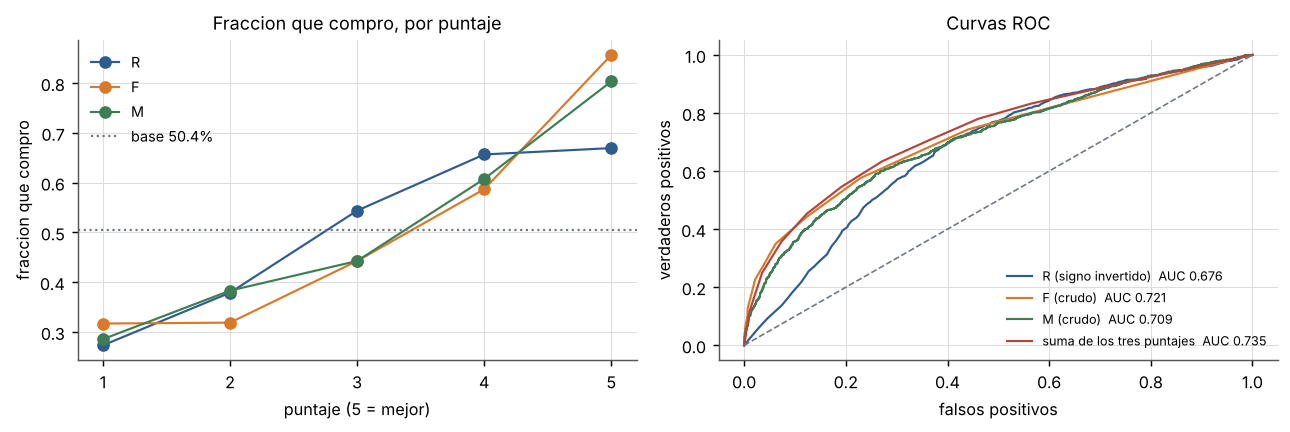
\includegraphics[width=\textwidth]{../figuras/p6_roc.png}
\caption{Izquierda: fracci\'on de clientes que compr\'o en la ventana,
seg\'un el puntaje de cada dimensi\'on. Derecha: curvas ROC con los valores
crudos. \textbf{Qu\'e muestra:} las tres dimensiones separan en la
direcci\'on correcta (m\'as puntaje, m\'as probabilidad de compra), pero F
es la de pendiente m\'as pronunciada. \textbf{Por qu\'e importa:} la
diferencia entre F y R no es sutil: el quintil top de F compra con
probabilidad \SI{85.7}{\percent} y el de R con \SI{66.9}{\percent}.}
\end{figure}

\paragraph{La respuesta: F.} Por las dos medidas:
\begin{itemize}[nosep,leftmargin=1.4em]
  \item \textbf{Por separaci\'on cruda}, la diferencia entre la fracci\'on
  que compra en el mejor y en el peor quintil es de \num{0.540} para F,
  \num{0.518} para M y \num{0.396} para R. F va de \SI{31.7}{\percent} en el
  puntaje~1 a \SI{85.7}{\percent} en el puntaje~5.
  \item \textbf{Por AUC}, F crudo da \num{0.7210}, M crudo \num{0.7093} y R
  con el signo invertido \num{0.6764}.
\end{itemize}

\begin{table}[htbp]
\centering
\footnotesize
\caption{\textbf{6.3} AUC de cada dimensi\'on, con los valores crudos (R con el signo invertido), y de la suma de los tres puntajes, como clasificadores de compra$_i$.}
\label{tab:p6_auc}
\begin{tabular}{lc}
\toprule
\textbf{clasificador} & \textbf{AUC} \\
\midrule
R (signo invertido) & 0.6764 \\
F (crudo) & 0.7210 \\
M (crudo) & 0.7093 \\
suma de los tres puntajes & 0.7352 \\
\bottomrule
\end{tabular}
\\[0.3em]{\scriptsize \textbf{Qu\'e leer:} la suma le gana a las tres por separado, que es la justificaci\'on emp\'irica de usar tres n\'umeros y no uno. La mejora es modesta porque las tres dimensiones est\'an correlacionadas entre s\'i.}
\end{table}


\paragraph{La suma de los tres puntajes gana a cualquiera por separado},
con AUC \num{0.7352}. La mejora sobre F sola es modesta (\num{0.014}), lo
cual es esperable porque las tres dimensiones est\'an correlacionadas entre
s\'i: un cliente que compra seguido tambi\'en compr\'o hace poco y gast\'o
m\'as. Pero la mejora existe, y es la justificaci\'on emp\'irica de por qu\'e
el RFM usa tres n\'umeros y no uno.

\paragraph{Un detalle que vale la pena notar sobre R.} La curva de R es la
m\'as plana de las tres \emph{en el extremo superior}: entre el puntaje~4
(\SI{65.7}{\percent}) y el~5 (\SI{66.9}{\percent}) casi no hay diferencia,
mientras que en F el salto del 4 al 5 es de \num{27} puntos porcentuales. La
raz\'on es que la recencia satura: una vez que un cliente compr\'o
``hace poco'', que haya sido hace tres d\'ias o hace diez no cambia mucho su
probabilidad de volver. F, en cambio, sigue discriminando hasta arriba,
porque un cliente con \num{139} facturas es cualitativamente distinto de uno
con \num{6}. Donde R s\'i funciona muy bien es en el extremo inferior: el
quintil menos reciente compra con probabilidad \SI{27.3}{\percent}, el m\'as
bajo de toda la tabla. R sirve para descartar, F para seleccionar.

\subsection{6.4 Los campeones}

Definiendo como \textbf{campeones} a los clientes con puntaje 4 o 5 en las
tres dimensiones:

\begin{table}[htbp]
\centering
\footnotesize
\caption{\textbf{6.4} Los campeones: clientes con puntaje 4 o 5 en las tres dimensiones.}
\label{tab:p6_campeones}
\begin{tabular}{lr}
\toprule
\textbf{concepto} & \textbf{valor} \\
\midrule
clientes campe\'ones (puntaje 4 o 5 en R, F y M) & 783 \\
fracci\'on de la base de clientes & 21.41\,\% \\
venta que generaron (\pounds) & 1\,302\,057.01 \\
venta total de la ventana, todos los clientes con ID (\pounds) & 2\,432\,839.69 \\
\textbf{fracci\'on de la venta de la ventana} & \textbf{53.52\,\%} \\
\bottomrule
\end{tabular}
\\[0.3em]{\scriptsize \textbf{Qu\'e leer:} el 21.4\,\% de los clientes genera el 53.5\,\% de la venta del trimestre. Es casi exactamente la ley de Pareto, y es el argumento comercial entero del RFM en una l\'inea.}
\end{table}


Son \textbf{\num{783} clientes}, el \SI{21.41}{\percent} de la base, y
generaron \textbf{\gbp\num{1302057}} de los \gbp\num{2432840} de venta neta
del 1 de octubre al 8 de diciembre de \emph{todos} los clientes con
\texttt{CustomerID}, incluidos los nuevos. Es decir, el
\SI{21.4}{\percent} de los clientes produce el \textbf{\SI{53.5}{\percent}}
de la venta.

Es casi exactamente la ley de Pareto, y es el argumento comercial entero del
an\'alisis RFM en una sola l\'inea: con tres n\'umeros por cliente, todos
calculados con informaci\'on disponible al 1 de octubre, se identifica a una
quinta parte de la base que vale la mitad del negocio del trimestre. Para un
equipo con presupuesto limitado de retenci\'on, saber a qui\'enes llamar
primero es casi todo el valor.

Conviene notar que el denominador es generoso con la comparaci\'on: incluye a
los clientes nuevos, que por construcci\'on no pod\'ian ser campeones. Contra
el total de los clientes que s\'i exist\'ian al 1 de octubre la fracci\'on
ser\'ia a\'un mayor.

\subsection{6.5 Los clientes nuevos y el l\'imite del enfoque}

\begin{table}[htbp]
\centering
\footnotesize
\caption{\textbf{6.5} Clientes sin ninguna factura de venta antes del 1 de octubre.}
\label{tab:p6_nuevos}
\begin{tabular}{lr}
\toprule
\textbf{concepto} & \textbf{valor} \\
\midrule
clientes nuevos en la ventana & 723 \\
venta que generaron (\pounds) & 382\,228.23 \\
\textbf{fracci\'on de la venta de la ventana} & \textbf{15.71\,\%} \\
\bottomrule
\end{tabular}
\\[0.3em]{\scriptsize \textbf{Qu\'e leer:} casi una sexta parte de la venta del trimestre viene de gente que el 1 de octubre no exist\'ia en la base. Ning\'un modelo cliente por cliente puede verlos, porque no tienen fila. El pron\'ostico agregado de la Parte~5 s\'i los incluye, sin saberlo.}
\end{table}


\paragraph{{\normalfont\itshape ¿Qu\'e fracci\'on de la venta vino de
clientes nuevos?}} \textbf{\num{723} clientes} compraron en la ventana sin
tener ninguna factura de venta antes del 1 de octubre, y generaron
\textbf{\gbp\num{382228}}, el \textbf{\SI{15.71}{\percent}} de la venta neta
del per\'iodo con \texttt{CustomerID}. Casi una sexta parte del negocio del
trimestre vino de gente que, el 1 de octubre, no exist\'ia en la base de
datos.

\paragraph{{\normalfont\itshape ¿Puede un an\'alisis RFM, o cualquier modelo
construido cliente por cliente, pronosticar esa venta?}} \textbf{No, y la
imposibilidad es estructural, no un problema de ajuste.} Un modelo cliente
por cliente necesita una fila por cliente para producir una predicci\'on. Los
\num{723} clientes nuevos \emph{no tienen fila} el 1 de octubre: no tienen
recencia (nunca compraron), no tienen frecuencia (cero facturas) ni monto. No
es que el modelo los prediga mal; es que no hay nada que meterle al modelo.
Ning\'un refinamiento del RFM, ni cambiar los quintiles, ni agregar
dimensiones, ni usar un modelo m\'as sofisticado, cambia eso. El techo de
cualquier enfoque bottom-up sobre esta base es el \SI{84.3}{\percent} de la
venta.

\paragraph{{\normalfont\itshape Con\'ectenlo con la Parte~5 y el
Proyecto~1.}} En el vocabulario de FPP2 \S10.3--10.4, la Parte~5 es un
pron\'ostico \textbf{top-down}: se pronostica el total agregado directamente,
sin preguntar qui\'en compra. Un modelo cliente por cliente es
\textbf{bottom-up}: se pronostica cada cliente y se suman las predicciones.

\textbf{¿Cu\'al de los dos puede ver a los clientes nuevos? El top-down, y
solo el top-down.} La raz\'on es que la serie agregada \emph{ya contiene} la
venta de los clientes nuevos sin necesidad de identificarlos: cuando S2 mira
la venta del 15 de noviembre, est\'a mirando un n\'umero que incluye tanto a
los clientes viejos como a los \num{723} nuevos, todos revueltos. El modelo
no sabe qui\'enes son, pero tampoco le hace falta: la tasa de llegada de
clientes nuevos es parte de la din\'amica que la serie agregada aprende de
forma impl\'icita, igual que aprende la estacionalidad semanal.

El enfoque bottom-up tiene la ventaja contraria: dice \emph{qui\'en}, que es
lo que se necesita para actuar (a qui\'en llamar, a qui\'en mandarle un
cup\'on). Pero paga ese detalle con un sesgo sistem\'atico hacia abajo, del
tama\~no exacto de la venta de los clientes nuevos, un \SI{15.7}{\percent} en
este trimestre.

La lectura para el Proyecto~1, donde se comparan ambos enfoques, es que la
comparaci\'on no deber\'ia ser solo de MAE. \textbf{Se espera que el
bottom-up pierda, y se sabe de antemano por cu\'anto y por qu\'e.} Lo
interesante ser\'a (i) si el bottom-up pierde \emph{m\'as} de ese
\SI{15.7}{\percent}, lo que indicar\'ia que adem\'as se equivoca con los
clientes que s\'i conoce; (ii) si corregir el pron\'ostico bottom-up con una
estimaci\'on separada de la llegada de clientes nuevos cierra la brecha; y
(iii) si el detalle por cliente compensa la p\'erdida de precisi\'on
agregada, que es una pregunta de negocio y no de estad\'istica. El h\'ibrido
natural (pronosticar el total con un modelo top-down y usar el RFM solo para
\emph{repartirlo} entre clientes) recoge lo mejor de ambos, y es la
reconciliaci\'on que FPP2 \S10.3--10.4 formaliza.

% ===========================================================================
\section{Conclusiones}
% ===========================================================================

\begin{enumerate}[leftmargin=1.6em]
  \item \textbf{La prueba que uno escoge decide lo que uno ve.} El proceso
  semanal de la Parte~0 no tiene ninguna memoria y pasa la prueba de
  rezago~1 el \SI{88.5}{\percent} de las veces, pero Ljung--Box con $m=10$ lo
  rechaza el \SI{95.5}{\percent}. Es el mismo problema de RANDU en la
  Tarea~2: pasar una prueba no es evidencia de ausencia de estructura.

  \item \textbf{Reprobar la prueba de ruido blanco casi nunca significa
  ``hay memoria''.} En estos datos la autocorrelaci\'on ven\'ia sobre todo de
  una media que no era constante: el d\'ia de la semana (un \'indice de
  \num{1.56} el jueves contra \num{0.57} el domingo) y la subida navide\~na.
  La receta de quitar primero y preguntar despu\'es funcion\'o.

  \item \textbf{La limpieza es una decisi\'on, no un procedimiento.} Las
  seis reglas eliminan \num{7930} filas, pero la decisi\'on que m\'as
  importa es una que \emph{no} elimina: conservar el c\'odigo \texttt{Manual},
  sin el cual la venta de \gbp\num{38970} del 10 de junio se queda sin su
  cancelaci\'on. Y el orden de las reglas cambia la bit\'acora aunque no
  cambie el resultado.

  \item \textbf{El calendario es parte del modelo.} Descubrir que la tienda
  cierra los s\'abados no es un dato de color: es lo que fija $s=6$, lo que
  explica por qu\'e el pico de la ACF est\'a en el rezago~6 y lo que hace que
  el promedio de los \'indices estacionales sea \num{1.20} y no~\num{1}.

  \item \textbf{El diagn\'ostico de residuos predijo al ganador.} S2 fue el
  \'unico modelo cuyos residuos pasaron Ljung--Box en 4.4, y fue el que
  gan\'o en prueba en 5.3. Lo que los dos resultados tienen en com\'un es la
  diferenciaci\'on: es lo que le permite a S2 seguir un nivel que sube, y es
  lo que hizo que no le quedara tendencia en los residuos.

  \item \textbf{Una validaci\'on solo protege contra la fuga que ocurre
  despu\'es de ella.} La media m\'ovil centrada mejora el error un
  \SI{10}{\percent} sin que ni la validaci\'on cruzada ni el origen m\'ovil
  se den cuenta, porque la fuga viaja dentro de una columna calculada antes
  del corte. La \'unica se\~nal fue que (c) resultaba imposible de calcular.

  \item \textbf{Hay un error que ninguna validaci\'on puede estimar.} El
  origen m\'ovil corrigi\'o alrededor de un \SI{10}{\percent} del optimismo
  de la validaci\'on cruzada, pero sigui\'o subestimando el error de prueba en
  un \SI{39}{\percent}, porque noviembre no se parece a mayo. Con un solo
  a\~no de datos esa parte no se puede medir desde adentro, y la
  estacionalidad anual no se puede siquiera identificar.

  \item \textbf{Detr\'as de la serie hay clientes, pero la serie sabe algo
  que los clientes no.} El RFM identifica al \SI{21.4}{\percent} de la base
  que genera el \SI{53.5}{\percent} de la venta, lo cual es enormemente
  \'util para actuar. Pero el \SI{15.7}{\percent} de la venta del trimestre
  vino de clientes que no exist\'ian el 1 de octubre, y a esos solo los ve el
  pron\'ostico agregado.
\end{enumerate}

% ===========================================================================
\begin{thebibliography}{9}
\bibitem{chen} D. Chen. \emph{Online Retail} [conjunto de datos]. UCI
Machine Learning Repository, 2015.
\url{https://archive.ics.uci.edu/dataset/352/online+retail}

\bibitem{rfm} D. Chen, S. L. Sain y K. Guo. Data mining for the online
retail industry: A case study of RFM model-based customer segmentation using
data mining. \emph{Journal of Database Marketing \& Customer Strategy
Management}, 19(3):197--208, 2012.

\bibitem{fpp2} R. J. Hyndman y G. Athanasopoulos. \emph{Forecasting:
Principles and Practice}, 2a ed. OTexts, Melbourne, 2018.
\url{https://otexts.com/fpp2/}

\bibitem{tsay} R. S. Tsay. \emph{Analysis of Financial Time Series}, 2a ed.
Wiley, 2005.

\bibitem{harvey} A. C. Harvey. \emph{Forecasting, Structural Time Series
Models and the Kalman Filter}. Cambridge University Press, 1989. (Base de la
implementaci\'on del SARIMA en \texttt{src/utils\_ts.py}.)
\end{thebibliography}

\end{document}
